\documentclass[11pt]{article}
\usepackage[margin=1in]{geometry}
\usepackage{amsmath,amssymb,amsthm,mathtools}
\usepackage{bm}
\usepackage{graphicx}
\usepackage{placeins}
\usepackage{tikz}
\usetikzlibrary{decorations.pathmorphing,calc,arrows.meta}
\usepackage[colorlinks=true,linkcolor=blue!55!black,citecolor=blue!55!black,urlcolor=blue!55!black]{hyperref}
\usepackage{xcolor}

\definecolor{psi}{RGB}{40,111,176}
\definecolor{tbr}{RGB}{193,50,50}

\newcommand{\Tr}{\operatorname{Tr}}
\newcommand{\ket}[1]{\lvert #1\rangle}
\newcommand{\bra}[1]{\langle #1\rvert}
\newcommand{\brak}[2]{\langle #1 | #2\rangle}
\newcommand{\PB}{P_{\mathrm B}}
\newcommand{\PiT}{\Pi_T}
\newcommand{\KT}{K_T}
\newcommand{\OT}{O_T}
\newcommand{\DT}{D_T}
\newcommand{\Bern}{\mathrm{Bern}}
\newcommand{\dg}{^{\dagger}}
\newcommand{\eS}{e^{S_0}}

\newtheorem*{claim}{Claim}

% Pedagogical asides.  Default OFF (paper version); set \pedagogicaltrue for the
% teaching version with plain-language asides and the reader's guide.
\newif\ifpedagogical
\pedagogicalfalse
\definecolor{pedcol}{RGB}{20,110,95}
\newcommand{\ped}[1]{\ifpedagogical\par\smallskip{\small\color{pedcol}%
  \leftskip=1.4em\rightskip=1.4em\noindent$\triangleright$~\textit{Plain-language aside.}~#1\par}%
  \par\smallskip\fi}

\title{\bf Fragile Fortuity:\\ The Gravity of BPS Overlaps in Supersymmetric SYK}
\author{}
\date{}

\begin{document}
\maketitle

\begin{abstract}
\noindent
The fortuitous BPS states of the $\mathcal N{=}2$ SYK model are strongly chaotic, and their
random--matrix description has recently been developed on the \emph{energy--spectrum} side. We
develop the complementary \emph{overlap} side. The uplift decoder $\OT=\PB\PiT\PB$, which measures the
metric fragility of BPS states across $N\!\to\!N{+}1$, is a Gram matrix of gravitational overlaps whose
disorder--averaged spectrum is the two--projector free--probability (Wachter/MANOVA) law---a
two--hard--edge (Jacobi) counterpart of the one--hard--edge (Bessel/Marchenko--Pastur) energy
models. We realize it as a Penington--Shenker--Stanford--Yang sum over end--of--the--world branes in
the topological ($E=0$) sector of $\mathcal N{=}2$ super--JT gravity: the genus expansion of the
overlap moments \emph{is} the gravitational sum over bulk topologies, the disk gives Wachter, and the
whole handle tower resums into a closed--form genus--one resolvent
$W_1(x)=-\gamma^2 x(x-1)/(a\,\sigma^5)$; the amplitude dictionary follows from the topological term
$e^{S_0\chi}$ of the action, so the gravity reproduces the handles to all orders. Two features escape
this universal description. \emph{(i)} A protected--atom resonance at $\lambda=0,1$---exactly
transmitted/lost BPS directions in excess of the ensemble---which is a finite--$N$ effect ($\sim\!5\%$
at $N\!=\!12$--$13$, vanishing by $N\!=\!14$), distinct from the robust $\mathbb Z_q$--Witten index
$3^{(N-1)/2}$. \emph{(ii)} A \emph{macroscopic soft tail}: the exact
decoder places an $O(10\%)$, non--vanishing fraction of BPS states below the Wachter hard edge, where
the ensemble (hence the wormhole sum) predicts none---a genuine breakdown of random--matrix
universality, distinct from the dilute sub--gap tunneling of the energy models. We trace this tail to
its origin: it is the smaller theory's near--BPS spectrum imaged into overlap variables by the uplift.
The map is an exact identity $\lambda=E/(E+\sigma_a^2)$ derived from the BPS constraint, which for
near--BPS energies is linear, $\lambda\simeq cE$ (correlation $0.95$, $c$ predicted from the couplings)
---the overlap shadow of the near--extremal throat, tying the tail directly to the energy--side model. Finally, the chaotic (fortuitous) states carry
Gaussian--unitary statistics while the monotone tower is deterministic, so the decoder separates
black--hole--microstate from graviton--gas content. The dual is one of \emph{gravitational overlaps},
not of spacetime geometry.
\end{abstract}

\tableofcontents
\bigskip

%======================================================================
\ifpedagogical
\section*{Reader's guide (plain language)}
\addcontentsline{toc}{section}{Reader's guide}
This paper mixes SYK, random--matrix theory, and 2d gravity. Teal asides throughout translate the
jargon; here is the core vocabulary in one place, using the one object everything is about---the
$d\times d$ decoder matrix $\OT=\PB\PiT\PB$, whose eigenvalues $\lambda\in[0,1]$ measure how well BPS
states survive an uplift.
\begin{itemize}\itemsep2pt
\item \textbf{Spectral measure $d\mu$ and moments $m_k$.} $d\mu$ is just the histogram of the
eigenvalues $\lambda$; the \emph{moments} are their averages $m_k=\frac1d\sum_i\lambda_i^k
=\frac1d\Tr\OT^k$. Knowing all $m_k$ is knowing the histogram.
\item \textbf{Resolvent $W(x)$.} A bookkeeping device that packages all moments into one function,
$W(x)=\frac1d\Tr\frac{1}{x-\OT}=\sum_k m_k/x^{k+1}$. Its singularities (a branch cut) mark where the
eigenvalues live; $m_{-1}=-W(0)$, etc. Physicists call it a resolvent, probabilists a Stieltjes
transform.
\item \textbf{Disorder average and genus expansion.} We average over the random SYK couplings. The
average moments organize as a series in $1/D=e^{-S_0}$ ($D=$ sector dimension): $\ m_k=m_k^{(0)}
+D^{-2}m_k^{(1)}+\cdots$. Each power of $D^{-2}$ is one ``handle'' on a surface---this is the
\emph{genus expansion}.
\item \textbf{Spectral curve / topological recursion.} The leading (disk) resolvent $W_0(x)$ is an
algebraic function---a curve. \emph{Topological recursion} is a machine that, fed only this curve,
cranks out every higher term $W_1,W_2,\dots$ by taking residues. \S\ref{sec:W1} and Appendix~A use
it to get $W_1$ in closed form.
\item \textbf{EOW branes / gravitational overlaps.} In the gravity picture the BPS states and the
slot are ``end--of--the--world branes''; the moments are computed by a gravitational path integral
summing 2d surfaces (Appendix~B). ``Wormhole'' $=$ a surface connecting two boundaries.
\end{itemize}
\fi

%======================================================================
\section{The decoder side}
\label{sec:decoder}

\subsection{Model and the uplift decoder}
We work with the generic one--flavor $\mathcal N{=}2$ SYK model in its wedge realization: the
Hilbert space is the exterior algebra $\mathcal H=\Lambda^\bullet(\mathbb C^N)$, graded by fermion
number $p$ with $\dim\mathcal H^p=\binom Np$, and the supercharge is wedging with a generic
$q$--form ($q=3$),
\begin{equation}
  Q = C\wedge(\cdot),\qquad C=\!\!\sum_{i<j<k}\!\! C_{ijk}\,e_i\wedge e_j\wedge e_k,\qquad Q^2=0,\quad
  H=\{Q,Q\dg\}.
\end{equation}
The BPS states are the harmonic representatives $\mathcal B^p=\ker Q\cap\ker Q\dg\subset\mathcal H^p$,
and $\PB=\sum_i\ket{\psi_i}\bra{\psi_i}$ is the orthogonal projector onto $\mathcal B$.

Fortuity concerns what happens to a BPS state when the theory is \emph{uplifted}
$N\to N'=N+1$: the couplings $C_{ijk}$ are inherited and independent new couplings
$C_{ij,N+1}$ are drawn. A BPS state of the smaller theory need not remain BPS. The
\emph{uplift decoder} measures how much of an old BPS multiplet survives inside the new BPS
space after reading a fixed occupation pattern. Concretely, all objects live on the charge--$p$ Fock
space $\mathcal H=\Lambda^{p}(\mathbb C^{N'})$ ($\dim\mathcal H=D$), and are built from two orthogonal
projectors on it: $\PB$, onto the BPS space $\mathcal B=\mathcal B_{N'}^{p}$ ($\dim=d$), and
$\PiT=1-n_{N'}$, onto the occupation sector (the ``slot'') $\mathcal V$ ($\dim=m$). The \emph{uplift
decoder} and its two Gram operators are
\begin{equation}
  \DT=\PiT\,\PB,\qquad
  \KT=\DT\DT\dg=\PiT\,\PB\,\PiT ,\qquad
  \OT=\DT\dg\DT=\PB\,\PiT\,\PB .
  \label{eq:decoderdef}
\end{equation}
All three are $D\times D$ operators on $\mathcal H$: $\KT$ is supported on the slot $\mathcal V$
(rank $m$), $\OT$ on the BPS space $\mathcal B$ (rank $d$), and they share the same nonzero spectrum.
We work throughout with $\OT=\PB\PiT\PB$---the slot projector $\PiT$ compressed between the BPS
projectors, an LMRS--type ``compressed projector'' with $0\preceq\OT\preceq1$---whose eigenvalues
$\lambda\in[0,1]$ are the squared cosines of the principal angles between $\mathcal B$ and $\mathcal V$:
$\lambda=1$ is a perfectly transmitted (fortuitous) direction, $\lambda=0$ a lost one, and the interior
$0<\lambda<1$ is fragile (metric--dependent) content. Reduced to an orthonormal BPS basis $\OT$ is the
$d\times d$ matrix we diagonalize (its slot--side twin $\KT$ carries the same nonzero eigenvalues). The
\emph{uplift fidelity} $F_T=\tfrac1d\Tr\OT=m_1$ and the fragility cost
$\kappa_T=m_{-1}-1=\int\lambda^{-1}\,d\mu-1$ are the low moments of its spectral measure $d\mu$.
\ped{``Principal angles'' between two subspaces generalize the angle between two lines: $\lambda=
\cos^2\theta$, so $\lambda=1$ means the two directions coincide (the state sits inside the slot---
perfectly transmitted) and $\lambda=0$ means they are orthogonal (the state has no overlap with the
slot---lost). The whole physics is the \emph{distribution} of these $\lambda$'s, i.e.\ the histogram
$d\mu$; the fidelity is its mean and the dressing cost its inverse--mean.}

\subsection{Microscopic form of the decoder from the supercharge}
\label{sec:micro}
The decoder admits an exact self--energy form directly in terms of the supercharge. Let $Q_N$ be the
old supercharge, $H_N=\{Q_N,Q_N\dg\}$ its Hamiltonian, and $G=H_N^{-1}$ on $(\ker H_N)^\perp$ (zero on
$\ker H_N$) the Hodge Green's operator, so that the old BPS projector is
\begin{equation}
  \PB \;=\; 1 - Q_N\,G\,Q_N\dg - Q_N\dg\,G\,Q_N .
  \label{eq:PB}
\end{equation}
Uplift $N\to N'=N+1$ and fix the enlarged charge $p$. Every state splits by the occupation of the new
mode $e\equiv e_{N'}$,
\begin{equation}
  \ket\Psi=\ket a+\ket b\wedge e,\qquad
  \ket a\in\Lambda^{p}(\mathbb C^{N})\ \text{(empty)},\quad
  \ket b\in\Lambda^{p-1}(\mathbb C^{N})\ \text{(occupied)},
  \label{eq:absplit}
\end{equation}
so that $\PiT=1-n_{N'}$ reads off the empty part, $\PiT\ket\Psi=\ket a$ and $\bra\Psi\PiT\ket\Psi=\|a\|^2$.
The uplifted supercharge splits accordingly, $Q_{N'}=Q_N+C'$, with $C'=(D\wedge e)\wedge(\cdot)$ the
injection built from the \emph{new} couplings $D=\sum_{i<j\le N}C_{ij,N'}\,e_i\wedge e_j$ (the part of
$Q_{N'}$ that moves the added mode). Sorting $Q_{N'}\ket\Psi$ and $Q_{N'}\dg\ket\Psi$ by the presence of
$e$ (with $e\wedge e=0$) and demanding both vanish gives four conditions,
\begin{equation}
  Q_N\ket a=0,\qquad Q_N\dg\ket b=0,\qquad Q_N\ket b=-\,D\wedge\ket a,\qquad Q_N\dg\ket a=-\,\iota_{\bar D}\ket b .
  \label{eq:bpsfour}
\end{equation}
The first two make $\ket a$ closed and $\ket b$ co--closed; the last two couple them through the new
couplings.

We eliminate $\ket b$. Writing $u\equiv D\wedge a=C'a\in\Lambda^{p+2}(\mathbb C^N)$, conditions
\eqref{eq:bpsfour}(ii)--(iii) read $Q_N\dg b=0$ and $Q_N b=-u$, so
$H_N b=Q_N\dg Q_N b=-Q_N\dg u$ and hence
\begin{equation}
  \ket b=-\,G\,Q_N\dg\,(D\wedge a).
  \label{eq:belim}
\end{equation}
The occupied weight then collapses to a \emph{single} resolvent insertion. Using $GH_N=1$ on the
(co--closed, non--harmonic) $\ket b$, then $H_N\ket b=Q_N\dg Q_N\ket b$, then $[G,Q_N]=0$ and $u=-Q_Nb$,
\begin{equation}
  \|b\|^2=\bra b G H_N\ket b=\bra{Q_N b}\,G\,\ket{Q_N b}=\bra a\,{C'}\dg G\,C'\,\ket a ,
  \label{eq:selfnorm}
\end{equation}
an exact identity: the occupied norm is the new couplings propagated through the old resolvent. Here
$C'=D\wedge(\cdot):\Lambda^p\to\Lambda^{p+2}$ and $G$ acts at the intermediate degree $p+2$.

The decoder eigenvalue is the empty fraction, so \eqref{eq:selfnorm} gives
\[
  \lambda=\frac{\bra\Psi\PiT\ket\Psi}{\|\Psi\|^2}
  =\frac{\|a\|^2}{\|a\|^2+\|b\|^2}
  =\frac{\|a\|^2}{\|a\|^2+\bra a{C'}\dg G\,C'\ket a}.
\]
Parametrizing the BPS space by its closed empty components $\ket a$---the physical norm is
$\|\Psi\|^2=\bra a\,(1+{C'}\dg G\,C')\,\ket a$ while the decoder measures $\|a\|^2$---the eigenproblem
$\OT\ket\Psi=\lambda\ket\Psi$ becomes $\ket a=\lambda\,(1+{C'}\dg G\,C')\,\ket a$, i.e.\ the exact
self--energy form
\begin{equation}
  \boxed{\;\OT=\big(1+{C'}\dg G\,C'\big)^{-1}\quad\text{on }\ker Q_N\subset\Lambda^p(\mathbb C^N)\;}
  \label{eq:KTself}
\end{equation}
with $G$ the old resolvent at degree $p+2$. This is a Schur--complement statement: the new mode leaks
the BPS state out of the BPS locus by the self--energy ${C'}\dg G\,C'$, and $\OT$ resums that leakage.
To leading order in the new couplings it is the familiar self--energy
$\OT=1-{C'}\dg G\,C'+\cdots$, with fidelity defect
$1-\OT={C'}\dg G\,C'/(1+{C'}\dg G\,C')\simeq{C'}\dg G\,C'$. Equation~\eqref{eq:KTself} is what makes the
disorder average tractable---$C'$ is Gaussian and independent of the inherited data---and it is the
operator form of the state--by--state identity $\lambda=E/(E+\sigma_a^2)$ of \S\ref{sec:tailorigin}
(with $\bra a{C'}\dg G\,C'\ket a/\|a\|^2=\sigma_a^2/E$). It is the microscopic object whose ensemble
statistics we now identify.

\subsection{A diagrammatic language}
\label{sec:diagrams}
The self--energy form \eqref{eq:KTself} invites a Feynman--diagram reading of the decoder
(Fig.~\ref{fig:feyn}). The rules are minimal: an external \emph{BPS leg} is on shell
($H_N\ket\psi=0$); the internal line is the \emph{off--BPS propagator} $G=1/H_N$, which vanishes on
the BPS locus so that only virtual excursions off it propagate; the new couplings enter through a
single \emph{vertex} $C'=D\wedge$ that knocks a BPS state off the locus by attaching the added mode;
and the inherited couplings enter through the old supercharge vertex $Q=C\wedge$. Reading left to
right, a state is kicked off the locus by $C'$, propagates by $G$, and is kicked back by ${C'}\dg$:
this is the self--energy $\Sigma={C'}\dg G\,C'$, and the decoder $\OT=(1+\Sigma)^{-1}$ resums the chain
of such blobs into a \emph{dressed BPS propagator},
\begin{equation}
  \OT=1-\Sigma+\Sigma^2-\cdots,\qquad 1-\OT\simeq\Sigma\quad(\text{leakage}).
  \label{eq:dyson}
\end{equation}
Even the BPS projector is of this form: \eqref{eq:PB} reads $\PB=1-Q\,G\,Q\dg-Q\dg G\,Q$, the identity
minus two self--energy blobs built from the old vertex $Q$.

Two features are transparent in this language. First, the \emph{soft tail is a resonance}: a
small--$\lambda$ state is a diagram whose internal $G$--line is itself near--BPS ($H_N\to0$), so
$G$---and hence $\Sigma$---diverges and $\lambda\to0$; the tail of \S\ref{sec:tailorigin} is a resonant
self--energy. Second, this is the \emph{microscopic}, single--realization companion of the ribbon/genus
expansion (\S\ref{sec:genus} onward): averaging over the Gaussian new couplings Wick--contracts the
$C'$ vertices pairwise, $\langle C'\,C'\rangle$, and each contraction is a ribbon edge, so
disorder--averaging these Feynman diagrams \emph{is} the fatgraph sum that the gravity reproduces. The
two tiers---Feynman diagrams before averaging, ribbons after---are related by that one contraction.

\begin{figure}[t]
\centering
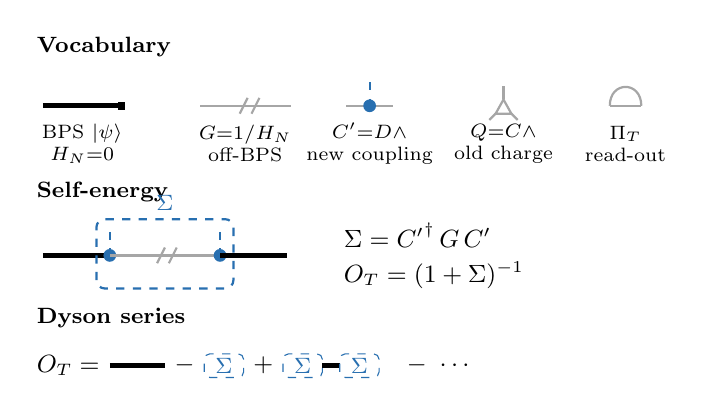
\begin{tikzpicture}[
  bps/.style={line width=1.9pt},
  prop/.style={line width=0.8pt,gray!70},
  nm/.style={psi,dashed,line width=0.7pt},
  vtx/.style={psi},
  L/.style={font=\footnotesize},
  S/.style={font=\scriptsize},
  op/.style={font=\small}]
% vocabulary row
\node[L,anchor=west] at (-0.2,2.35) {\textbf{Vocabulary}};
\draw[bps] (0,1.6)--(0.95,1.6);
\fill (0.95,1.55) rectangle +(0.09,0.1);
\node[S,align=center] at (0.5,1.12) {BPS $\ket\psi$\\ $H_N{=}0$};
\draw[prop] (2.0,1.6)--(3.15,1.6);
\draw[prop] (2.5,1.5)--(2.6,1.7);
\draw[prop] (2.65,1.5)--(2.75,1.7);
\node[S,align=center] at (2.57,1.12) {$G{=}1/H_N$\\ off-BPS};
\draw[nm] (4.15,1.9)--(4.15,1.6);
\draw[prop] (3.85,1.6)--(4.45,1.6);
\fill[vtx] (4.15,1.6) circle (2.3pt);
\node[S,align=center] at (4.15,1.12) {$C'{=}D\wedge$\\ new coupling};
\draw[prop] (5.75,1.5)--(5.95,1.5)--(5.85,1.68)--cycle;
\draw[prop] (5.85,1.68)--(5.85,1.85);
\draw[prop] (5.75,1.5)--(5.67,1.42);
\draw[prop] (5.95,1.5)--(6.03,1.42);
\node[S,align=center] at (5.85,1.12) {$Q{=}C\wedge$\\ old charge};
\draw[prop] (7.2,1.6) .. controls (7.2,1.92) and (7.6,1.92) .. (7.6,1.6);
\draw[prop] (7.2,1.6)--(7.6,1.6);
\node[S,align=center] at (7.4,1.12) {$\PiT$\\ read-out};
% self-energy
\node[L,anchor=west] at (-0.2,0.5) {\textbf{Self-energy}};
\draw[bps] (0,-0.3)--(0.85,-0.3);
\draw[nm] (0.85,0.0)--(0.85,-0.3);
\fill[vtx] (0.85,-0.3) circle (2.3pt);
\draw[prop] (0.85,-0.3)--(2.25,-0.3);
\draw[prop] (1.45,-0.4)--(1.55,-0.2);
\draw[prop] (1.6,-0.4)--(1.7,-0.2);
\draw[nm] (2.25,0.0)--(2.25,-0.3);
\fill[vtx] (2.25,-0.3) circle (2.3pt);
\draw[bps] (2.25,-0.3)--(3.1,-0.3);
\draw[psi,dashed,line width=0.8pt,rounded corners=3pt] (0.68,-0.72) rectangle (2.42,0.16);
\node[psi,font=\footnotesize] at (1.55,0.37) {$\Sigma$};
\node[op,anchor=west] at (3.7,-0.05) {$\Sigma={C'}\dg\,G\,C'$};
\node[op,anchor=west] at (3.7,-0.55) {$\OT=(1+\Sigma)^{-1}$};
% Dyson
\node[L,anchor=west] at (-0.2,-1.1) {\textbf{Dyson series}};
\node[op,anchor=west] at (-0.2,-1.7) {$\OT=$};
\draw[bps] (0.85,-1.7)--(1.55,-1.7);
\node[op] at (1.8,-1.7) {$-$};
\draw[psi,dashed,rounded corners=2pt] (2.05,-1.85) rectangle (2.55,-1.55);
\node[psi,font=\footnotesize] at (2.3,-1.7) {$\Sigma$};
\node[op] at (2.8,-1.7) {$+$};
\draw[psi,dashed,rounded corners=2pt] (3.05,-1.85) rectangle (3.55,-1.55);
\node[psi,font=\footnotesize] at (3.3,-1.7) {$\Sigma$};
\draw[bps] (3.55,-1.7)--(3.77,-1.7);
\draw[psi,dashed,rounded corners=2pt] (3.77,-1.85) rectangle (4.27,-1.55);
\node[psi,font=\footnotesize] at (4.02,-1.7) {$\Sigma$};
\node[op,anchor=west] at (4.5,-1.7) {$-\ \cdots$};
\end{tikzpicture}
\caption{A Feynman--diagram language for the uplift decoder. \emph{Top:} the vocabulary---BPS external
legs (on shell, $H_N{=}0$), the off--BPS propagator $G{=}1/H_N$, the new--coupling vertex
$C'{=}D\wedge$ (attaching the added mode, dashed), the inherited supercharge vertex $Q{=}C\wedge$, and
the slot read--out $\PiT$. \emph{Middle:} the self--energy insertion $\Sigma={C'}\dg G\,C'$; the
decoder is its resummation $\OT=(1+\Sigma)^{-1}$. \emph{Bottom:} equivalently $\OT$ is the Dyson
series \eqref{eq:dyson}, a dressed BPS propagator. Disorder--averaging Wick--contracts the $C'$
vertices into the ribbon edges of \S\ref{sec:genus}; a near--BPS internal line ($H_N\to0$) is the
resonance that produces the soft tail.}
\label{fig:feyn}
\end{figure}

\subsection{The disorder--averaged law: Wachter/MANOVA}
Because $C'$ is independent Gaussian and the BPS subspace is (numerically) Haar--typical inside
the charge sector, the disorder--averaged spectrum of $\OT$ is the compression of one projector
by an independent random subspace: a \emph{Jacobi (MANOVA)} ensemble. With
\begin{equation}
  D=\binom{N+1}{p}\ \ (\text{sector dim}),\qquad
  d=\dim\mathcal B=\widetilde D_p-\widetilde D_{\,N+1-p-q}\ \ (\text{index}),\qquad
  m=\binom{N}{p},
\end{equation}
and the two ratios $a=d/D$, $b=m/D=(N{+}1{-}p)/(N{+}1)$, the interior density is the
\emph{Wachter law}
\begin{equation}
  \rho_0(\lambda)=\frac{\sqrt{(\lambda_+-\lambda)(\lambda-\lambda_-)}}{2\pi\,a\,\lambda(1-\lambda)},
  \qquad
  \lambda_\pm=\big(\sqrt{a(1-b)}\pm\sqrt{b(1-a)}\big)^2 ,
  \label{eq:wachter}
\end{equation}
supplemented by atoms $p_0=\max(0,1-b/a)$ at $\lambda=0$ and $p_1=\max(0,1-(1-b)/a)$ at
$\lambda=1$. Here $\widetilde D_M(k)=\sum_n(-1)^n\binom{M}{k-qn}$ is the twisted counting function,
and the closed form for $a$ is the fortuity index itself.

Equivalently, $\rho_0$ is the free multiplicative convolution of two Bernoulli laws,
$\Bern(a)\boxtimes\Bern(b)$ (Voiculescu freeness of the two projectors). Its $S$--transform
factorizes, $S(z)=\tfrac{(1+z)^2}{(a+z)(b+z)}$, giving all moments in closed form:
\begin{equation}
  m_1=b,\quad m_2=b(a+b-ab),\quad m_3=b\big(a^2+b^2+3ab-3a^2b-3ab^2+2a^2b^2\big),\ \dots
  \label{eq:moments}
\end{equation}
with the full generating function fixed by the algebraic (genus--zero) spectral curve
\begin{equation}
  (w-1)\,z^2+\big(w(a+b)-1\big)\,z+w\,ab=0 ,\qquad z=\psi(w)=\textstyle\sum_k M_k w^k,\ \ m_k=M_k/a .
  \label{eq:curve}
\end{equation}
\ped{Three names for one fact. ``Free multiplicative convolution $\boxtimes$'' is the rule that
gives the eigenvalue histogram of a product of two \emph{generic} (freely rotated) matrices from the
two factor histograms---here two projectors, of relative sizes $a$ and $b$. The ``$S$--transform''
is the tool that makes $\boxtimes$ into ordinary multiplication (like $\log$ turns products into
sums), which is why the moments come out in closed form. And ``spectral curve'' is just the equation
\eqref{eq:curve} that the moment generating function solves---an algebraic curve because it is a
quadratic. All three encode the same disk--level Wachter law.}
Exact diagonalization confirms \eqref{eq:wachter}--\eqref{eq:moments} in the bulk across
$N=6,\dots,10$ (Kolmogorov--Smirnov distance $\lesssim0.1$, tightening with $N$); the mean
$\langle\lambda\rangle=b$ is an exact trace identity at every $N$
(Figs.~\ref{fig:density}--\ref{fig:cdf}).

\begin{figure}[!htb]
\centering
\includegraphics[width=\textwidth]{decoder_wachter_density.pdf}
\caption{Interior decoder spectrum from exact diagonalization (blue histogram, pooled over disorder
realizations) versus the analytic Wachter density \eqref{eq:wachter} (black), for the one--flavor
down channel at half filling, $N=6,\dots,9$. The parameters $a,b$ are fixed by the closed--form
dimensions (no fitting); the bulk Kolmogorov--Smirnov distance is $\lesssim0.1$ and the endpoint
atom weights track the Wachter predictions $p_0,p_1$. The interior fills the band $[\lambda_-,
\lambda_+]$ with the characteristic $U$--shape.}
\label{fig:density}
\end{figure}

\begin{figure}[!htb]
\centering
\includegraphics[width=\textwidth]{decoder_wachter_cdf.pdf}
\caption{The same comparison as empirical CDF (blue) versus the Wachter CDF (dashed), cleaner at the
edges, for the one--flavor down channel $N=6\!\to\!7,\dots,10\!\to\!11$. Agreement tightens with $N$
(KS falling to $\sim0.05$); the residual near $\lambda=0,1$ is the protected excess beyond the
Wachter atoms.}
\label{fig:cdf}
\end{figure}

\subsection{The protected part: a finite--$N$ resonance}
Two channels of the spectrum are \emph{not} fragile and not captured by \eqref{eq:wachter}: exact atoms
at $\lambda=1$ (states in $\mathcal B_N^{p}\cap\ker C'$, transmitted exactly) and at $\lambda=0$ (states
in $\mathcal B_N^{p-1}\cap\ker {C'}\dg$, lost exactly), disorder--independent and in excess of the
Wachter atoms $p_0,p_1$. Their exact counts $n_1=\dim(\mathcal B_N^{p}\cap\ker C')$ and
$n_0=\dim(\mathcal B_N^{p-1}\cap\ker {C'}\dg)$ are a \emph{finite--$N$ resonance}: they are appreciable
only where $\dim\mathcal B_N^p\approx\binom{N}{p+2}$, near $N=12$--$13$, and vanish once the two
separate. The total atom fraction $(n_0+n_1)/d$ is $5.6\%$ at $N=12$ and $N=13$ but \emph{zero} at
$N=14,15,16$ (each over two disorder realizations): once $\dim\mathcal B_N^p\sim(\sqrt3)^N$ drops below
$\binom{N}{p+2}\sim2^N/\sqrt N$ with a growing margin, $C'$ acts injectively on $\mathcal B_N^p$ and no
exact atoms survive. The protected core is thus a small transient, not a robust sector; the finite--$N$
atoms dissolve into the near--edge tail as $N$ grows, in keeping with the collapse of the band in
\S\ref{sec:largeN}.

Distinct from these atoms is the $\mathbb Z_q$--twisted Witten index, a robust object. The enlarged BPS
dimension is $d=3^{\lfloor N/2\rfloor}$ (times $2$ for odd $N$; \S\ref{sec:largeN}), so the BPS entropy
density is exactly $\tfrac12\ln3$; in the two--flavor tower the protected BPS dimension obeys
\begin{equation}
  \dim\mathcal B^m_{2m+1}=3^m
  \quad\Longleftrightarrow\quad
  S_0=\tfrac{N-1}{2}\ln 3 ,
  \label{eq:index}
\end{equation}
proved by a generating--function/Lagrange--B\"urmann collapse. This index counts BPS states and sets the
extremal entropy; it is \emph{not} the decoder's exact--atom count $n_0+n_1$ above, which it exceeds by
an order of magnitude already at $N=12$. With that distinction the spectrum splits as
\begin{equation}
  \underbrace{\rho_0(\lambda)\ \text{(Wachter)}}_{\text{fragile / chaotic bulk}}
  \;+\;
  \underbrace{\text{a finite--}N\text{ atom resonance at }\lambda=0,1}_{\text{transient; }0\text{ for }N\ge14} ,
  \label{eq:split}
\end{equation}
and the object of this paper is a bulk (gravitational) account of the fragile part, with the protected
atoms as its transient finite--$N$ complement.

\FloatBarrier
%======================================================================
\section{The genus expansion of the decoder}
\label{sec:genus}

The finite--$D$ moments are exact and carry a topological grading. Writing
$\OT=\PB\PiT\PB$ with $\PB=VV\dg$ for a Haar $D\times d$ isometry $V$, so that
$\Tr\OT^{\,k}=\Tr(V\dg\PiT V)^{k}$, the Weingarten calculus
gives, with $\gamma=(1\,2\,\cdots\,k)$ the cyclic permutation and $c(\cdot)$ the number of cycles,
\begin{equation}
  \big\langle\Tr \OT^{\,k}\big\rangle
  =\sum_{\sigma,\tau\in S_k}\mathrm{Wg}(\sigma\tau^{-1};D)\;
  m^{\,c(\sigma)}\;d^{\,c(\gamma^{-1}\tau)} ,
  \qquad m_k=\tfrac1d\big\langle\Tr\OT^{\,k}\big\rangle .
  \label{eq:weingarten}
\end{equation}
\ped{``Weingarten calculus'' is just the formula for the average of a product of matrix entries of a
random unitary $U$: the answer is a sum over pairings of the $U$'s with the $\bar U$'s, indexed by
two permutations $\sigma,\tau$, weighted by the Weingarten function $\mathrm{Wg}$. It is the exact,
finite--$D$ version of Wick's theorem for the unitary group. Each pairing is a ``ribbon graph''
(a thickened Feynman diagram); how twisted it is---its genus---fixes its power of $1/D$.}
Each term is a ribbon graph whose Euler characteristic sets its power of $1/D$; expanding in
$1/D=e^{-S_0}$ organizes the moment by genus,
\begin{equation}
  m_k = m_k^{(0)}(a,b) + \frac{1}{D^2}\,m_k^{(1)}(a,b) + \frac{1}{D^4}\,m_k^{(2)}(a,b)+\cdots
  \label{eq:genus}
\end{equation}
The genus--zero (planar) piece is exactly the Wachter law \eqref{eq:moments}. The genus--one
(single--handle) pieces are, in closed form,
\begin{align}
  m_1^{(1)}&=0, \\
  m_2^{(1)}&=-\,b(1-a)(1-b), \label{eq:m2handle}\\
  m_3^{(1)}&=\phantom{-}b(1-a)(1-b)\,(10ab-5a-5b+1), \label{eq:m3handle}\\
  m_4^{(1)}&=-\,5\,b(1-a)(1-b)\,(14a^2b^2-14a^2b+3a^2-14ab^2+10ab-a+3b^2-b). \label{eq:m4handle}
\end{align}
The first moment receives no handle---$m_1=b$ exactly, all orders---and every nonzero handle carries
the common prefactor $b(1-a)(1-b)$, which vanishes when the subspace or slot fills the sector
($a$ or $b\to1$): no room for topology. Equations \eqref{eq:m2handle}--\eqref{eq:m4handle} are the
targets the gravity side must reproduce. They have been checked against Haar Monte Carlo: e.g.\ at
$a=b=\tfrac12$, $m_2=\tfrac38-\tfrac14 D^{-2}$, $m_3=\tfrac5{16}-\tfrac3{16}D^{-2}$, and
$m_4=\tfrac{35}{128}-\tfrac{15}{64}D^{-2}$, all matching to $O(D^{-4})$. The alternating signs and
shared prefactor already hint that the whole tower resums to a single object, which we exhibit in
\S\ref{sec:W1}.

\subsection{Chord diagrams and the Narayana count}
\label{sec:chords}
The same expansion has a gravity--native reading as a sum over bulk worldlines---\emph{chord
diagrams}---on the disk, the technology used for near--BPS operator spectra and Berry curvature in
super--JT~\cite{LMRS,Berry}. Each factor of $\PiT$ in $m_k=\tfrac1a\,\tau\big((\PB\PiT)^k\big)$ is a
boundary insertion; the disk amplitude sums over bulk chords joining them, planar (non--crossing) chords
being genus zero and crossings the handles, suppressed by $e^{-2S_0}=1/D^2$---exactly the grading
\eqref{eq:genus}.

\smallskip\noindent\emph{Where the planar limit comes from.} In the operator computations
of~\cite{LMRS,Berry} the non--crossing (free) regime is reached by sending the inserted operator's
dimension $\Delta\to\infty$, which exponentially suppresses crossed worldlines. We have no such
$\Delta$; its role is played by the large--sector--entropy planar limit $D=e^{S_0}\to\infty$,
equivalently the Haar--typicality of the BPS subspace (\S\ref{sec:decoder}). There the two projectors
$\PB$ and $\PiT$ are asymptotically \emph{free} (Voiculescu), so non--crossing diagrams dominate and
crossings are the finite--$D$ handles. The soft tail (\S\ref{sec:softtail}) is exactly where this
freeness fails---the BPS subspace is not Haar--typical along the near--BPS directions---so it lies
outside the chord expansion, matching \S\ref{sec:tailorigin}.

\smallskip\noindent\emph{Catalan vs.\ Narayana.} The nature of the insertion is decisive. A heavy
\emph{Gaussian} operator $\hat\Lambda=\PB\Lambda\PB$ contracts pairwise, so its non--crossing diagrams
are non--crossing \emph{pairings}, counted by the Catalan numbers $C_k=\tfrac1{k+1}\binom{2k}{k}$ and
giving the \emph{semicircle}~\cite{LMRS,Berry}. Our insertion $\PiT$ is a \emph{projector},
$\PiT^2=\PiT$: a chord may enclose an entire run of insertions at no cost, so the non--crossing diagrams
are non--crossing \emph{partitions}, counted by the Narayana numbers
\begin{equation}
  \mathrm{Nar}(k,c)=\tfrac1k\binom{k}{c}\binom{k}{c-1},\qquad \sum_{c=1}^{k}\mathrm{Nar}(k,c)=C_k ,
  \label{eq:narayana}
\end{equation}
the refinement of the Catalan count by the number of blocks $c$ (Fig.~\ref{fig:chords}). Weighting each
partition by the free cumulants of the two Bernoulli spectra $\Bern(a),\Bern(b)$ and summing gives their
free multiplicative convolution---the Wachter moments \eqref{eq:moments}---while the reference--block
self--consistency (a chosen block cuts the disk into independent sub--disks) reproduces the quadratic
spectral curve \eqref{eq:curve}. The two--hard--edge Wachter law is thus the Narayana (projector)
counterpart of the single--edge semicircle (Catalan/Gaussian), and reinstating crossings restores the
handle tower \eqref{eq:m2handle}--\eqref{eq:m4handle}.

\smallskip\noindent\emph{The moments, explicitly.} For two free projectors the disk moments are the
non--crossing--partition sum
\begin{equation}
  m_k=\frac1a\sum_{\pi\in\mathrm{NC}(k)}\Big(\prod_{V\in\pi}\kappa_{|V|}\Big)\,b^{\,|K(\pi)|},
  \qquad \kappa_1=a,\ \ \kappa_2=a(1{-}a),\ \ \kappa_3=a(1{-}a)(1{-}2a),\ \dots
  \label{eq:ncmoments}
\end{equation}
the $\kappa_s$ being the free cumulants of $\Bern(a)$ and $K(\pi)$ the Kreweras complement
($|K(\pi)|=k{+}1{-}|\pi|$): each block of $\pi$ is a $\psi$--index loop weighted by its cumulant, each
block of $K(\pi)$ a $t$--index loop weighted by $b$. This \emph{is} the planar necklace
\eqref{eq:necklace}---a non--crossing partition is a planar ribbon graph---with $\kappa_2=a(1{-}a)$
packaging the two--disk and planar--wormhole surfaces of \S\ref{sec:grav} into one block. Enumerating
the partitions (Fig.~\ref{fig:ncpart}),
\begin{align*}
  m_1&=\tfrac1a\,\kappa_1 b=b,\\
  m_2&=\tfrac1a\big(\kappa_1^2 b+\kappa_2 b^2\big)=ab+(1{-}a)b^2=b(a+b-ab),\\
  m_3&=\tfrac1a\big(\kappa_1^3 b+3\,\kappa_2\kappa_1 b^2+\kappa_3 b^3\big)
      =b\big(a^2+b^2+3ab-3a^2b-3ab^2+2a^2b^2\big),
\end{align*}
reproducing \eqref{eq:moments} term by term---the same disk values the gravitational sum gives in
\S\ref{sec:grav} (the factor $3$ in $m_3$ is the three two--block partitions
$\{12\}\{3\},\,\{23\}\{1\},\,\{13\}\{2\}$).

\smallskip\noindent\emph{The handles: one crossing.} Reinstating crossings promotes a non--crossing
partition to a genus--one configuration, each crossing costing one handle, $1/D^2$. Already at $k=2$
the exact finite--$D$ moment is rational and shows both orders at once,
\begin{equation}
  m_2=\frac{b\big[D^2(a+b-ab)-1\big]}{D^2-1}
     =\underbrace{b(a+b-ab)}_{\text{disk}}\;-\;\underbrace{b(1-a)(1-b)}_{m_2^{(1)}}\,\frac1{D^2}+O(D^{-4}),
  \label{eq:m2exact}
\end{equation}
so the single crossing diagram of Fig.~\ref{fig:cross}---the wormhole whose $\psi$-- and $t$--chords
must cross, i.e.\ the handle---together with the $1/D^2$ dressings of the planar terms gives
$m_2^{(1)}=-b(1-a)(1-b)$, matching \eqref{eq:m2handle}. The same crossing sum at $k=3$ gives
$m_3^{(1)}=b(1-a)(1-b)(10ab-5a-5b+1)$, and the once--crossing partitions, weighted by the subleading
Weingarten, reproduce the entire handle tower \eqref{eq:m2handle}--\eqref{eq:m4handle}---which we have
verified symbolically through $m_4$. The chord diagrams thus generate \emph{both} the disk
(non--crossing, Narayana/Wachter) and the handles (crossing): an exact alternative to the surface sum
of \S\ref{sec:grav}.

\begin{figure}[t]
\centering
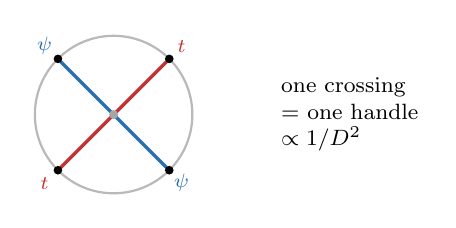
\begin{tikzpicture}[
  bdot/.style={circle,fill=black,inner sep=1.1pt},
  arc/.style={line width=1.2pt}]
  \draw[gray!55,line width=0.8pt] (0,0) circle (1.0);
  \coordinate (p1) at (135:1.0);\coordinate (p2) at (45:1.0);
  \coordinate (p3) at (-45:1.0);\coordinate (p4) at (-135:1.0);
  \draw[arc,psi] (p1)--(p3);
  \draw[arc,tbr] (p2)--(p4);
  \fill[gray!70] (0,0) circle (1.6pt);
  \node[bdot] at (p1){};\node[bdot] at (p2){};\node[bdot] at (p3){};\node[bdot] at (p4){};
  \node[psi,font=\scriptsize] at (135:1.24){$\psi$};
  \node[tbr,font=\scriptsize] at (45:1.22){$t$};
  \node[psi,font=\scriptsize] at (-45:1.22){$\psi$};
  \node[tbr,font=\scriptsize] at (-135:1.24){$t$};
  \node[font=\footnotesize,align=left] at (3.0,0)
    {one crossing\\ $=$ one handle\\ $\propto 1/D^2$};
\end{tikzpicture}
\caption{The genus--one handle as a crossing chord diagram ($k=2$): the $\psi$--chord (blue) and
$t$--chord (red) cross (gray dot), and each crossing is a handle weighting $1/D^2$. Summed at each $k$
with the subleading Weingarten, the crossing diagrams give the handle tower
\eqref{eq:m2handle}--\eqref{eq:m4handle} and hence \eqref{eq:m2exact} at $k=2$.}
\label{fig:cross}
\end{figure}

\begin{figure}[t]
\centering
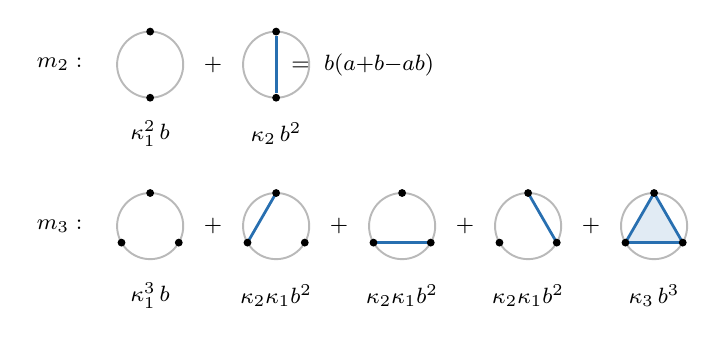
\begin{tikzpicture}[
  bdot/.style={circle,fill=black,inner sep=1.0pt},
  chord/.style={psi,line width=1.0pt},
  dsk/.style={gray!55,line width=0.7pt},
  wt/.style={font=\footnotesize}]
\node[wt] at (0.05,0) {$m_2:$};
\begin{scope}[shift={(1.2,0)}]
  \draw[dsk](0,0) circle(0.42);
  \node[bdot] at (90:0.42){}; \node[bdot] at (270:0.42){};
  \node[wt] at (0,-0.88) {$\kappa_1^2\,b$};
\end{scope}
\node[wt] at (2.0,0) {$+$};
\begin{scope}[shift={(2.8,0)}]
  \draw[dsk](0,0) circle(0.42);
  \node[bdot](t) at (90:0.42){}; \node[bdot](bb) at (270:0.42){};
  \draw[chord] (t)--(bb);
  \node[wt] at (0,-0.88) {$\kappa_2\,b^2$};
\end{scope}
\node[wt] at (3.9,0) {$=\ b(a{+}b{-}ab)$};
\node[wt] at (0.05,-2.05) {$m_3:$};
\begin{scope}[shift={(1.2,-2.05)}]
  \draw[dsk](0,0) circle(0.42);
  \node[bdot] at (90:0.42){}; \node[bdot] at (210:0.42){}; \node[bdot] at (330:0.42){};
  \node[wt] at (0,-0.88) {$\kappa_1^3\,b$};
\end{scope}
\node[wt] at (2.0,-2.05) {$+$};
\begin{scope}[shift={(2.8,-2.05)}]
  \draw[dsk](0,0) circle(0.42);
  \coordinate(a1) at (90:0.42);\coordinate(a2) at (210:0.42);\coordinate(a3) at (330:0.42);
  \draw[chord] (a1)--(a2);
  \node[bdot] at (a1){};\node[bdot] at (a2){};\node[bdot] at (a3){};
  \node[wt] at (0,-0.88) {$\kappa_2\kappa_1 b^2$};
\end{scope}
\node[wt] at (3.6,-2.05) {$+$};
\begin{scope}[shift={(4.4,-2.05)}]
  \draw[dsk](0,0) circle(0.42);
  \coordinate(c1) at (90:0.42);\coordinate(c2) at (210:0.42);\coordinate(c3) at (330:0.42);
  \draw[chord] (c2)--(c3);
  \node[bdot] at (c1){};\node[bdot] at (c2){};\node[bdot] at (c3){};
  \node[wt] at (0,-0.88) {$\kappa_2\kappa_1 b^2$};
\end{scope}
\node[wt] at (5.2,-2.05) {$+$};
\begin{scope}[shift={(6.0,-2.05)}]
  \draw[dsk](0,0) circle(0.42);
  \coordinate(e1) at (90:0.42);\coordinate(e2) at (210:0.42);\coordinate(e3) at (330:0.42);
  \draw[chord] (e1)--(e3);
  \node[bdot] at (e1){};\node[bdot] at (e2){};\node[bdot] at (e3){};
  \node[wt] at (0,-0.88) {$\kappa_2\kappa_1 b^2$};
\end{scope}
\node[wt] at (6.8,-2.05) {$+$};
\begin{scope}[shift={(7.6,-2.05)}]
  \draw[dsk](0,0) circle(0.42);
  \coordinate(f1) at (90:0.42);\coordinate(f2) at (210:0.42);\coordinate(f3) at (330:0.42);
  \fill[psi!14] (f1)--(f2)--(f3)--cycle;
  \draw[chord] (f1)--(f2)--(f3)--cycle;
  \node[bdot] at (f1){};\node[bdot] at (f2){};\node[bdot] at (f3){};
  \node[wt] at (0,-0.88) {$\kappa_3\,b^3$};
\end{scope}
\end{tikzpicture}
\caption{The non--crossing partitions generating the disk moments via \eqref{eq:ncmoments}. Blue chords
group the $\psi$--insertions into blocks (a block of size $s$ weights $\kappa_s$; singletons carry no
chord), and the complementary $t$--loops weight $b$ each. Summing the two diagrams for $m_2$ and the
five for $m_3$ gives the Wachter moments \eqref{eq:moments}; crossings (not shown) add the $1/D^2$
handles.}
\label{fig:ncpart}
\end{figure}

\begin{figure}[t]
\centering
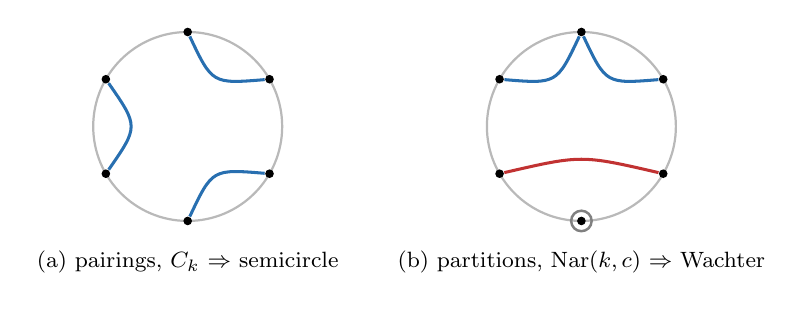
\begin{tikzpicture}[scale=1.0,
  bdot/.style={circle,fill=black,inner sep=1.1pt},
  arc/.style={line width=1.1pt}]
% (a) pairings / Catalan
\begin{scope}[shift={(0,0)}]
  \draw[gray!55,line width=0.8pt] (0,0) circle (1.2);
  \foreach \A/\n in {90/1,30/2,-30/3,-90/4,-150/5,150/6}{\node[bdot](a\n) at (\A:1.2){};}
  \draw[arc,psi] (a1) .. controls (0.312,0.54) .. (a2);
  \draw[arc,psi] (a3) .. controls (0.312,-0.54) .. (a4);
  \draw[arc,psi] (a5) .. controls (-0.623,0) .. (a6);
  \node at (0,-1.72) {\footnotesize (a) pairings, $C_k$ $\Rightarrow$ semicircle};
\end{scope}
% (b) partitions / Narayana
\begin{scope}[shift={(5,0)}]
  \draw[gray!55,line width=0.8pt] (0,0) circle (1.2);
  \foreach \A/\n in {90/1,30/2,-30/3,-90/4,-150/5,150/6}{\node[bdot](b\n) at (\A:1.2){};}
  \draw[arc,psi] (b6) .. controls (-0.312,0.54) .. (b1);
  \draw[arc,psi] (b1) .. controls (0.312,0.54) .. (b2);
  \draw[arc,tbr] (b3) .. controls (0,-0.36) .. (b5);
  \draw[gray,line width=0.9pt] (b4) circle (0.13);
  \node at (0,-1.72) {\footnotesize (b) partitions, $\mathrm{Nar}(k,c)$ $\Rightarrow$ Wachter};
\end{scope}
\end{tikzpicture}
\caption{Disk chord diagrams for the decoder moments. \emph{(a)} A Gaussian insertion contracts
pairwise, so the planar diagrams are non--crossing \emph{pairings} (Catalan $C_k$)---the semicircle
case of \cite{LMRS,Berry}. \emph{(b)} The projector $\PiT$ ($\PiT^2=\PiT$) lets one chord enclose a
whole block, so the planar diagrams are non--crossing \emph{partitions} (Narayana $\mathrm{Nar}(k,c)$;
here the blocks $\{1,2,6\}$ blue, $\{3,5\}$ red, and the singleton $\{4\}$), giving the two--hard--edge
Wachter law. Crossings, not drawn, are the $1/D^2$ handles.}
\label{fig:chords}
\end{figure}

\smallskip\noindent\emph{Relation to the Berry--curvature computation.} Reference~\cite{Berry} applies
this same chord technology in $\mathcal N{=}2$ super--JT to a different overlap observable: the Berry
curvature $F_{\mu\nu}=i[\hat\Lambda_\mu,\hat\Lambda_\nu]$ of the moduli--space connection, a commutator
of two projected \emph{Gaussian} operators, whose spectrum is the free commutator of two semicircles.
Our decoder $\OT=\PB\PiT\PB$ is a compression of two \emph{projectors}, giving the two--edge
Wachter/Narayana law, and its ensemble breaks down through the macroscopic soft tail
(\S\ref{sec:softtail}), which has no counterpart in the edge--regular commutator spectrum. The two are
complementary overlap--side chaos diagnostics for fortuitous BPS states, computed by the same super--JT
machinery.

\subsection{The cylinder and the spectral form factor}
\label{sec:sff}
The disk gave the moments; the \emph{cylinder}---two trace boundaries joined through the bulk---gives the
connected double--trace moments $\langle\Tr\OT^m\,\Tr\OT^n\rangle_c$ and hence the spectral form factor.
In chord language these are annular non--crossing partitions on the two boundaries~\cite{Berry};
equivalently they are the universal two--point resolvent (the ``double trumpet'') of the Wachter spectral
curve,
\begin{equation}
  W_{0,2}(x_1,x_2)=\frac{1}{2(x_1-x_2)^2}\!\left[\frac{x_1x_2-\tfrac{\lambda_-+\lambda_+}{2}(x_1{+}x_2)+\lambda_-\lambda_+}{\sigma(x_1)\,\sigma(x_2)}-1\right],\quad \sigma(x)=\sqrt{(x-\lambda_-)(x-\lambda_+)}.
  \label{eq:cylinder}
\end{equation}
\begin{center}
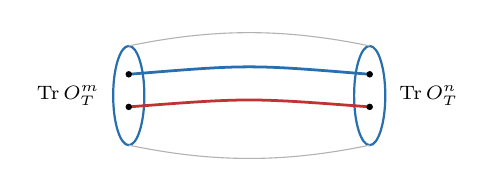
\begin{tikzpicture}[scale=0.9]
  \draw[psi,thick] (0,0) ellipse (0.22 and 0.7);
  \draw[psi,thick] (3.4,0) ellipse (0.22 and 0.7);
  \draw[gray!60] (0,0.7) .. controls (1.2,0.95) and (2.2,0.95) .. (3.4,0.7);
  \draw[gray!60] (0,-0.7) .. controls (1.2,-0.95) and (2.2,-0.95) .. (3.4,-0.7);
  \draw[psi,line width=1pt] (0,0.30) .. controls (1.7,0.44) .. (3.4,0.30);
  \draw[tbr,line width=1pt] (0,-0.16) .. controls (1.7,-0.03) .. (3.4,-0.16);
  \fill (0,0.30) circle(1.3pt);\fill(3.4,0.30) circle(1.3pt);
  \fill (0,-0.16) circle(1.3pt);\fill(3.4,-0.16) circle(1.3pt);
  \node[font=\scriptsize,left] at (-0.28,0){$\Tr\OT^m$};
  \node[font=\scriptsize,right] at (3.68,0){$\Tr\OT^n$};
\end{tikzpicture}
\end{center}
This $W_{0,2}$ is \emph{universal}---fixed by the two hard edges $\lambda_\pm$ alone, independent of the
potential; it is the genus--zero, two--boundary object of the same topological recursion that produced
$W_1$ in App.~\ref{sec:W1}. Its double discontinuity across the cut is the connected density correlator,
whose smooth part is the universal sine kernel
$\langle\rho(\lambda)\rho(\lambda')\rangle_c\sim-1/[2\pi^2(\lambda-\lambda')^2]$, which Fourier
transforms to a linear ramp. With the auxiliary--time form factor
$\mathrm{SFF}_c(t)=\langle\Tr e^{i\OT t}\,\Tr e^{-i\OT t}\rangle_c$, the cylinder gives the
Gaussian--unitary ramp and plateau,
\begin{equation}
  \mathrm{SFF}_c(t)\;\simeq\;\frac{t}{2\pi}\quad(\text{ramp}),\qquad
  \mathrm{SFF}_c\to d\ \ \text{at the Heisenberg time }\ t_H=2\pi d\ (\text{plateau}) .
  \label{eq:ramp}
\end{equation}
Exact diagonalization of the Jacobi ensemble confirms this over two decades (Fig.~\ref{fig:sff}): an
initial dip, a ramp of fitted slope $0.159\approx1/2\pi$, then the plateau at $d$. This is the
\emph{smooth--correlator} face of the chaos already seen discretely in $\langle r\rangle=$ GUE
(\S\ref{sec:interp}): the decoder's overlap spectrum carries random--matrix correlations throughout its
Wachter band. The ramp is the same super--JT cylinder that produces the energy--side and
Berry--curvature~\cite{Berry} form factors; only the boundary observable differs (two projectors, hence
the Wachter curve and its two edges in \eqref{eq:cylinder}). It is unaffected by the soft tail---a disk
(density) feature, whereas the ramp is the connected cylinder---consistent with the tail being
non--universal in density but GUE in correlations (\S\ref{sec:interp}).

\begin{figure}[t]
\centering
\includegraphics[width=0.7\textwidth]{sff_ramp.pdf}
\caption{The decoder spectral form factor from exact diagonalization of the Jacobi ensemble
($a{=}b{=}\tfrac12$, $d=300$, pooled over $240$ realizations): dip, then the Gaussian--unitary ramp
$t/2\pi$ (black line), then the plateau $\mathrm{SFF}_c=d$ at the Heisenberg time $t_H=2\pi d$. The
overlap spectrum is random--matrix correlated throughout its band---the smooth--correlator counterpart
of the adjacent--gap result $\langle r\rangle=$ GUE.}
\label{fig:sff}
\end{figure}

%======================================================================
\section{The gravitational model}
\label{sec:grav}

\subsection{Two brane species in the topological sector}
In the West--Coast / PSSY model~\cite{PSSY} JT gravity is decorated with EOW branes whose flavor
index labels black--hole microstates; the disorder--averaged Gram matrix of the microstates is a
random matrix, and connected \emph{replica wormholes} generate its off--diagonal statistics, so
that its spectrum is Marchenko--Pastur and its rank is bounded by
$e^{S_0}$~\cite{MP,DistinguishMicro}. We use the same machinery with \emph{two} brane species:
\begin{itemize}
\itemsep2pt
\item $\psi$--branes carrying the $d$ BPS flavors ($\ket{\psi_i}$, $i=1,\dots,d$);
\item $t$--branes carrying the $m$ flavors of the slot, $\PiT=\sum_{\alpha=1}^m\ket{t_\alpha}\bra{t_\alpha}$.
\end{itemize}
\ped{An ``end--of--the--world (EOW) brane'' is a boundary condition where the 2d geometry simply
ends, carrying a label (``flavor'')---here, which BPS state or which slot state. In PSSY they encode
black--hole microstates. The key rule (made precise in \S\ref{sec:action}) is that a brane
conserves its flavor along its length, so summing over the flavor around a closed brane loop just
counts the states: $d$ for a $\psi$--loop, $m$ for a $t$--loop.}
A decoder moment is then a \emph{necklace} of gravitational overlaps,
\begin{equation}
  \Tr(\PB\PiT)^k
  =\sum_{\{i_a\}}\sum_{\{\alpha_a\}}
  \brak{\psi_{i_1}}{t_{\alpha_1}}\!\brak{t_{\alpha_1}}{\psi_{i_2}}\!
  \brak{\psi_{i_2}}{t_{\alpha_2}}\cdots\brak{t_{\alpha_k}}{\psi_{i_1}} ,
  \label{eq:necklace}
\end{equation}
and the gravitational path integral instructs us to sum over all ways bulk geometry glues the
$2k$ overlap edges. Because the BPS states sit at $E=0$, the $\mathcal N{=}2$ super--Schwarzian is
frozen onto its index $\delta(E)$: there is \emph{no propagating energy}, only the topological
brane combinatorics. This is precisely why the dual is one of \emph{overlaps}, not geometry.

\subsection{Amplitudes and Feynman rules}
The topological sector supplies a minimal set of amplitudes:
\begin{center}
\begin{tabular}{ll}
\emph{disk} & $Z_1=\eS=D$ \quad(sector degeneracy)\\[2pt]
\emph{wormhole tube} & weight $\dfrac{1}{D^2-1}=\dfrac{1}{D^2}\displaystyle\sum_{h\ge0}D^{-2h}$
\quad(one handle per factor $e^{-2S_0}$)\\[8pt]
\emph{$\psi$--index loop} & factor $d=aD$\\[2pt]
\emph{$t$--index loop} & factor $m=bD$\\[2pt]
\emph{genus--$g$ surface} & net suppression $D^{-2g}$
\end{tabular}
\end{center}
The exact Weingarten kernel is the all--handle resummation of the wormhole tube, so
\eqref{eq:weingarten} \emph{is} the gravitational sum over topologies for \eqref{eq:necklace}.

\subsection{Why the disk is Wachter: the 't Hooft mechanism}
A single connected wormhole costs $1/D^2$, but the $\psi$-- and $t$--flavor loops threading it pay
$m\,d\sim ab\,D^2$, exactly compensating. Hence \emph{all planar wormholes are unsuppressed} and
must be resummed; the resummation is a Schwinger--Dyson equation identical to the free
subordination equation for $\Bern(a)\boxtimes\Bern(b)$---the algebraic curve \eqref{eq:curve}---and
its solution is the Wachter density \eqref{eq:wachter}. PSSY's Marchenko--Pastur law is the dilute
limit $b\to0$ (a rare slot $=$ few branes) of this two--parameter law. Only geometries with an
\emph{uncompensated} handle survive at order $1/D^2$.

\subsection{The four bulk surfaces of $m_2$}
For $k=2$ the sum over gluings yields exactly four ribbon graphs, Fig.~\ref{fig:m2}. Three are
planar and one carries a handle:
\begin{center}
\begin{tabular}{clcc}
\hline
$(\sigma,\tau)$ & topology & genus & weight\\
\hline
$(e,e)$ & two disks (disconnected) & $0$ & $b^2$\\
$(e,\text{swap})$ & planar $\psi$--wormhole $+\,t$--loop & $0$ & $-ab^2$\\
$(\text{swap},\text{swap})$ & connected wormhole & $0$ & $ab$\\
$(\text{swap},e)$ & \textbf{handle} & $1$ & $-b/D^2$\\
\hline
\end{tabular}
\end{center}
\ped{``Ribbon graph'' and ``genus,'' concretely. Draw the four ways the two $\psi$--branes and two
$t$--branes can be paired up and fatten the lines into ribbons; each way is a little surface. Three
of them lie flat in the plane (genus $0$, no handles); the fourth can only be drawn by letting a
ribbon cross over itself, which forces a handle (genus $1$). The genus is literally the number of
handles, and each handle costs a factor $1/D^2$.}
The genus--zero surfaces sum to $b^2-ab^2+ab=b(a+b-ab)=m_2^{(0)}$, the Wachter disk. The handle,
together with the $O(1/D^2)$ curvature dressings of the three planar surfaces, sums to
\begin{equation}
  m_2^{(1)} = -\,b(1-a)(1-b) ,
\end{equation}
matching \eqref{eq:m2handle} exactly. This is the gravity side producing the first handle from an
honest sum over topologies.

\begin{figure}[t]
\centering
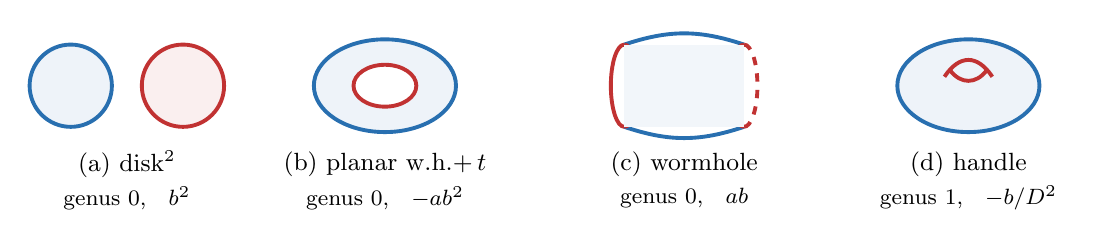
\begin{tikzpicture}[scale=0.95,
  brane/.style={line width=1.4pt},
  psiln/.style={brane,psi}, tbrln/.style={brane,tbr},
  cap/.style={line width=1pt,gray!70}]

% (a) two disks
\begin{scope}[shift={(0,0)}]
  \fill[psi!8] (0.0,0) circle(0.55);
  \fill[tbr!8] (1.5,0) circle(0.55);
  \draw[psiln] (0.0,0) circle(0.55);
  \draw[tbrln] (1.5,0) circle(0.55);
  \node at (0.75,-1.05) {\small (a) disk$^2$};
  \node at (0.75,-1.5) {\footnotesize genus $0$, \; $b^2$};
\end{scope}

% (b) planar wormhole + t loop  (annulus with an inner loop)
\begin{scope}[shift={(4.2,0)}]
  \fill[psi!8] (0,0) ellipse (0.95 and 0.62);
  \fill[white] (0,0) ellipse (0.42 and 0.28);
  \draw[psiln] (0,0) ellipse (0.95 and 0.62);
  \draw[tbrln] (0,0) ellipse (0.42 and 0.28);
  \node at (0,-1.05) {\small (b) planar w.h.$+\,t$};
  \node at (0,-1.5) {\footnotesize genus $0$, \; $-ab^2$};
\end{scope}

% (c) connected wormhole (cylinder)
\begin{scope}[shift={(8.2,0)}]
  \draw[psiln] (-0.8,0.55) .. controls (-0.2,0.75) and (0.2,0.75) .. (0.8,0.55);
  \draw[psiln] (-0.8,-0.55) .. controls (-0.2,-0.75) and (0.2,-0.75) .. (0.8,-0.55);
  \draw[tbrln] (-0.8,0.55) arc (90:270:0.18 and 0.55);
  \draw[tbrln,dashed] (-0.8,0.55) arc (90:-90:0.18 and 0.55);
  \draw[tbrln] (0.8,0.55) arc (90:270:0.18 and 0.55);
  \draw[tbrln,dashed] (0.8,0.55) arc (90:-90:0.18 and 0.55);
  \fill[psi!6] (-0.8,-0.55) rectangle (0.8,0.55);
  \node at (0,-1.05) {\small (c) wormhole};
  \node at (0,-1.5) {\footnotesize genus $0$, \; $ab$};
\end{scope}

% (d) handle (torus with boundary)
\begin{scope}[shift={(12.0,0)}]
  \fill[psi!8] (0,0) ellipse (0.95 and 0.62);
  \draw[psiln] (0,0) ellipse (0.95 and 0.62);
  % handle
  \draw[tbrln] (-0.32,0.12) .. controls (-0.12,0.42) and (0.12,0.42) .. (0.32,0.12);
  \draw[tbrln] (-0.24,0.20) .. controls (-0.10,0.02) and (0.10,0.02) .. (0.24,0.20);
  \node at (0,-1.05) {\small (d) handle};
  \node at (0,-1.5) {\footnotesize genus $1$, \; $-b/D^2$};
\end{scope}

\end{tikzpicture}
\caption{The four bulk surfaces contributing to $m_2$. Blue ($\psi$) and red ($t$) mark the two
brane species. Panels (a)--(c) are planar (genus $0$) and resum to the Wachter disk
$b(a+b-ab)$; the flavor loops on the connected wormhole (c) compensate its $1/D^2$ cost, so it is
unsuppressed. Panel (d) is the single uncompensated \textbf{handle}; with the curvature dressings of
(a)--(c) it yields $m_2^{(1)}=-b(1-a)(1-b)$.}
\label{fig:m2}
\end{figure}

\subsection{$m_3$: the same machine, next order}
At $k=3$ the gluing sum produces $12$ planar surfaces, $21$ leading genus--one surfaces, and $3$
genus--two surfaces. Grouped by topology,
\begin{align}
  m_3^{(0)}&=b\big(a^2+b^2+3ab-3a^2b-3ab^2+2a^2b^2\big)\quad(\text{disk, Wachter}),\\
  m_3^{(1)}&=b(1-a)(1-b)(10ab-5a-5b+1)\quad(\text{handle}),
\end{align}
both reproduced exactly by the topological expansion, in agreement with
\eqref{eq:m3handle}. The leading coefficient of $m_k$ is the Catalan number $C_{k-1}$
(the Fuss--Catalan fingerprint of freeness), providing an independent check that the disk is the
free convolution. The check extends to $m_4$ (agreeing with \eqref{eq:m4handle}, verified against
Haar data), with the disk keeping its Catalan leading coefficient $C_3=5$.

\subsection{The genus--one resolvent in closed form}
\label{sec:W1}
The whole handle tower resums to a single meromorphic form.
\ped{Topological recursion, in one breath: it is a machine (Eynard--Orantin) that takes the disk data
of a curve---here the Wachter resolvent $W_0$ and its two branch points---and produces \emph{every}
higher genus term by a fixed residue formula, no new input needed. Below we quote its output for
genus one; Appendix~\ref{app:W1} carries out the residues step by step. ``$\omega_{1,1}$'' is its
name for the genus--one, one--point function, which is just $W_1(x)\,dx$.}
Applying Eynard--Orantin topological
recursion~\cite{EO} to the Wachter spectral curve---uniformized by Zhukovsky
$x(z)=\alpha+\gamma(z+z^{-1})$ with branch points at $z=\pm1$, disk data
$y(z)-y(1/z)=-\sigma(x)/\big(a\,x(1-x)\big)$, and $\gamma^2=ab(1-a)(1-b)$, $\alpha=a+b-2ab$---the
genus--one one--point function $\omega_{1,1}$ (spelled out in Appendix~\ref{app:W1}) evaluates to
\begin{equation}
  \boxed{\;
  W_1(x)\;=\;-\,\frac{b(1-a)(1-b)\,x(x-1)}{\big[(x-\lambda_-)(x-\lambda_+)\big]^{5/2}}
  \;=\;-\,\frac{\gamma^2\,x(x-1)}{a\,\sigma(x)^5}\;}
  \label{eq:W1}
\end{equation}
where $W_1(x)=\sum_{k\ge2}m_k^{(1)}/x^{k+1}$ and $\sigma(x)=\sqrt{(x-\lambda_-)(x-\lambda_+)}$. The
single normalization subtlety---the $\tfrac1D\Tr$ versus $\tfrac1d\Tr$ bookkeeping between the
$D\times D$ matrix and the $d\times d$ compression---enters as an overall factor $-1/a^2$, fixed
exactly at six independent $(a,b)$ points. Expanding \eqref{eq:W1} at large $x$ regenerates
\eqref{eq:m2handle}--\eqref{eq:m4handle} identically, and predicts
\begin{multline}
  m_5^{(1)} = 5\,b(1-a)(1-b)\big(84a^3b^3-126a^3b^2+56a^3b-7a^3-126a^2b^3+154a^2b^2\\
  {}-49a^2b+3a^2+56ab^3-49ab^2+8ab-7b^3+3b^2\big).
\end{multline}

Three features confirm \eqref{eq:W1} is the genuine genus--one object rather than a fit:
\emph{(i)} its only singularities are at the branch points $\lambda_\pm$; in the local coordinate
$\zeta$ with $x-\lambda_\pm\sim\zeta^2$, the differential $W_1\,dx\sim\zeta^{-4}d\zeta$ is a pole of
order $6g-4+2n=4$ with no residue---the universal structure of $\omega_{1,1}$.
\emph{(ii)} The numerator $x(x-1)$ vanishes at the hard walls $\lambda=0,1$, so the handle
contributes \emph{nothing} at the protected--atom locations: the wormhole tower never touches the
fortuity core, now visible in the analytic structure of $W_1$ itself.
\emph{(iii)} The common prefactor $b(1-a)(1-b)$ of all handle moments is manifest as the overall
coefficient, and the resolvent's genus--one correction is purely odd across the cut (no rational
part), so a single line encodes the entire alternating--sign tower.

%======================================================================
\section{The amplitude dictionary from the super--JT action}
\label{sec:action}

So far the amplitudes of \S\ref{sec:grav} were \emph{adopted} from the matrix--integral duality.
We now argue that in the BPS sector they instead \emph{follow} from the $\mathcal N{=}2$ super--JT
action, and that this simultaneously settles the all--genus statement.

\subsection{The action and its topological term}
The $\mathcal N{=}2$ super--JT action for a surface $\Sigma$ is
\begin{equation}
  I \;=\; \underbrace{-S_0\,\chi(\Sigma)}_{\text{topological}}
  \;+\; I_{\text{super--Sch}}[\partial\Sigma]
  \;+\; I_{\text{brane}}[\text{EOW}],
  \qquad
  -S_0\chi=-\frac{S_0}{2\pi}\Big(\tfrac12\!\int_\Sigma\!\sqrt g\,R+\!\int_{\partial\Sigma}\!\!\sqrt h\,K\Big),
  \label{eq:action}
\end{equation}
the last equality being Gauss--Bonnet. The topological term alone weights every connected surface by
\begin{equation}
  e^{-I_{\text{top}}}=e^{S_0\chi(\Sigma)} .
  \label{eq:eSchi}
\end{equation}
This is exact and requires no dynamical input: it is simply the value of the Einstein--Hilbert term
in two dimensions.

\subsection{Why the dressing trivializes: the decoder is kinematic}
In general JT the full amplitude is \eqref{eq:eSchi} \emph{dressed} by the (super--)Schwarzian path
integral---the disk is $e^{S_0}Z_{\text{Sch}}(\beta)$, the cylinder is a nontrivial
double--trumpet, and so on. The dressing carries all the finite--energy dynamics. The decoder,
however, is built \emph{entirely from zero--energy states}: $\PB$ projects onto the BPS subspace,
and $\OT=\PB\PiT\PB$ is a purely kinematic operator on it. A gravitational quantity that depends
only on the BPS Hilbert space cannot depend on the Schwarzian dynamics that governs finite $E$; it
can only see the topological sector. Concretely, the super--Schwarzian density of states is
$\rho(E)=e^{S_0}\delta(E)+\rho_{\text{cont}}(E)$ with a gap~\cite{HITZ,N2matrix,BPSmicro};
projecting each boundary to $E=0$ keeps only the $\delta(E)$, whose weight is the degeneracy
$e^{S_0}$.
\ped{The ``super--Schwarzian'' is the theory that lives on the boundary of super--JT; its density of
states $\rho(E)$ tells you how many states sit at each energy. The picture is a spike of $e^{S_0}$
exactly--zero--energy (BPS) states---the $\delta(E)$---then a gap, then an ordinary continuum. Our
decoder only ever asks about the spike, so all the continuum dynamics drops out and only the count
$e^{S_0}$ remains. That is what ``the dressing trivializes'' means.} Thus the dressing on every BPS--projected boundary collapses to the number $e^{S_0}$, and
the amplitude of a surface reduces to its topological value \eqref{eq:eSchi}:
\begin{equation}
  Z(\Sigma)\big|_{\text{BPS}} \;=\; e^{S_0\chi(\Sigma)}\times(\text{brane flavor traces}).
  \label{eq:ZBPS}
\end{equation}
At the disk this is the exact BPS degeneracy $Z_1=e^{S_0}$~\cite{HITZ,BPSmicro}; the statement for
higher topology is the kinematic (energy--independent) extension, consistent with the super--JT
matrix--model structure~\cite{N2matrix}.

\subsection{Branes and the assembly}
The two projectors enter as two EOW--brane species: $\psi$--branes ($d$ BPS flavors) for $\PB$ and
$t$--branes ($m$ flavors) for $\PiT$, exactly the microstate branes whose overlaps the gravitational
path integral computes~\cite{BPSmicro,PSSY}. A brane segment conserves its flavor index, so a closed
$\psi$--loop contributes $\sum_{i=1}^d 1=d$ and a closed $t$--loop $m$; distinct species share no
disk, connecting only through wormholes. With $e^{S_0}=D$ and $\chi=2-2g-(\#\text{boundaries})$,
Eq.~\eqref{eq:ZBPS} gives immediately
\begin{equation}
  \text{disk }(\chi{=}1):\ e^{S_0}=D,\qquad
  \text{each handle}:\ e^{-2S_0}=D^{-2},\qquad
  \psi\text{--loop}:\ d,\quad t\text{--loop}:\ m,
\end{equation}
which is precisely the amplitude dictionary of \S\ref{sec:grav}---now read off the action rather than
imposed.

\subsection{All genus, and the unification}
The gravitational path integral sums \eqref{eq:ZBPS} over all fillings of a moment's brane necklace.
By the standard 't~Hooft/fatgraph duality---the $D$--power of a ribbon graph equals the Euler
characteristic of its dual surface---this sum is \emph{identically} the Weingarten average
\eqref{eq:weingarten}.
\ped{This is the hinge of the whole argument. On the matrix side (Weingarten), each diagram comes with a
power of $D$; on the gravity side, each surface comes with $e^{S_0\chi}=D^{\chi}$. 't~Hooft's 1974
observation is that these are the \emph{same} number---the power of $D$ from the index loops of a
fattened diagram equals the Euler characteristic of the surface you get by filling the diagram in.
So ``sum over random--matrix diagrams'' and ``sum over 2d surfaces'' are two names for one sum, and
the genus expansion of the moments \emph{is} the gravitational sum over topologies.} Hence the action reproduces the entire genus expansion: the disk is the
Wachter law, genus one is the closed form $W_1$ of \eqref{eq:W1}, and every handle follows. The three
descriptions coincide,
\begin{equation}
  \boxed{\ \text{super--JT action }e^{S_0\chi}\ \Longleftrightarrow\
  \text{Weingarten genus expansion}\ \Longleftrightarrow\
  \text{topological recursion on \eqref{eq:curve}}\ }
\end{equation}
and ``the action reproduces the handles to all orders'' holds because the BPS sector is
\emph{topological}: there is no separate dynamical wormhole to evaluate. The handle coefficients are
purely combinatorial (fatgraph counts)---which is exactly why they were computable from Weingarten
and resummable into $W_1$---while the action's sole contribution, the weight $e^{S_0\chi}$, is exact.

\subsection*{Status of the derivation}
\emph{Derived (exact):} the weight $e^{S_0\chi}$ from the topological term; the flavor traces from
the brane boundary conditions; hence the dictionary, the genus counting, and---via the fatgraph
duality---the all--genus reproduction of the Wachter law and $W_1$. \emph{Derived in the
literature:} the disk degeneracy $Z_1=e^{S_0}$ and the BPS--microstate overlap/Gram--matrix
construction~\cite{HITZ,BPSmicro,N2matrix}. \emph{Assumed:} that BPS localization trivializes the
super--Schwarzian dressing at all genus (proved at the disk; argued here from the kinematic nature of
the decoder and the super--JT matrix--model structure), and the sum--over--topologies as the
gravitational path integral. \emph{Genuinely open:} the extension \emph{off} the BPS point, $E\neq0$,
where the Schwarzian dynamics no longer trivializes and reproducing the amplitudes would require a
true dynamical super--JT computation. At $E=0$ the derivation is complete; away from it lies the
frontier.

%======================================================================
\section{Where the ensemble fails: the macroscopic soft tail}
\label{sec:softtail}

The gravitational/ensemble description of \S\ref{sec:grav}--\ref{sec:action} reproduces every
positive moment $m_{k\ge1}$ of the decoder. It does \emph{not} reproduce the exact spectrum near
$\lambda=0$, and the discrepancy is not small.

\paragraph{A macroscopic, non--Haar tail.}
Exact diagonalization in the large--$N$ ($a<b$) regime places a population of BPS states \emph{below}
the Wachter hard edge $\lambda_-$, extending down to $\lambda\sim10^{-4}$--$10^{-5}$
(Fig.~\ref{fig:softtail}, left). A Haar--random subspace at the identical $(D,d,m)$ has \emph{zero}
sub--edge eigenvalues (checked at every $N$), so the tail is genuinely non--Haar: invisible to the
free--probability law and to the wormhole sum built on it. Crucially it is \emph{macroscopic}---an
$O(10\%)$ fraction of all BPS states ($9\%,9\%,15\%,14\%$ at $N=12$--$15$; Fig.~\ref{fig:softtail},
right)---and it \emph{grows} as $a=d/D$ decreases (i.e.\ with $N$), from $\simeq9\%$ at $a=0.42$ to
$\simeq15\%$ at $a=0.34$. Two controls confirm this is the tail growing, not the edge sliding: the
\emph{deep}--tail fraction (states below $\lambda_-/5$, insensitive to small edge shifts) rises in
step ($4\%\to6\%$), while the Kolmogorov--Smirnov distance of the \emph{bulk} $[\lambda_-,\lambda_+]$
to the Wachter law stays flat ($0.08\to0.07$). So the bulk is universal and improving, and the tail
is the non--universal excess, growing. This is a genuine breakdown of random--matrix universality for
the fortuitous overlap spectrum, not a finite--size or dilute effect.

\paragraph{What the tail is.}
The decoder eigenvalue is exactly $\lambda=\bra{\psi}(1-n_{N'})\ket{\psi}$, so the small--$\lambda$
states are BPS states concentrated on the \emph{newly added mode being occupied}---the
``almost--lost'' content. The tail is the structured, near--boundary part of the fortuity window that
the generic (Haar) model cannot see.

\paragraph{The dressing cost is edge--sensitive, not a runaway.}
Because $\kappa=\int\lambda^{-1}d\mu-1$ is dominated by the smallest $\lambda$, it is controlled by
this tail. But $\kappa$ is \emph{not} a clean function of $N$: it peaks where the ensemble edge itself
approaches zero (near the $a=b$ line) and is otherwise moderate ($\kappa=115,282,44,45$ at $N=12$--$15$).
The robust, universal diagnostic of the breakdown is the tail \emph{fraction}, not $\kappa$; the
early ``$\kappa$ runs away'' reading was an artifact of sampling near criticality.

\begin{figure}[!htb]
\centering
\includegraphics[width=\textwidth]{soft_tail.pdf}
\caption{\emph{Left:} exact decoder spectra ($N=12,13$) leak an $O(10\%)$ fraction of states below the
Wachter edge $\lambda_-$ (dotted), down to $\lambda\sim10^{-5}$; a Haar--random subspace at the same
$(D,d,m)$ has no sub--edge weight (dashed). \emph{Right:} both the tail fraction ($\lambda<\lambda_-$)
and the deep--tail fraction ($\lambda<\lambda_-/5$) grow with $N$, while the bulk stays Wachter (KS
$0.08\to0.07$) and the Haar sub--edge weight is $0\%$ throughout. The growing tail is the part of the
fortuitous overlap spectrum that the RMT/gravity ensemble misses.}
\label{fig:softtail}
\end{figure}

\paragraph{Status.} \emph{Firm} (over $N=12$--$15$): the tail exists, is non--Haar (Haar gives $0\%$
at every $N$), is macroscopic, and \emph{grows}---in both the total and the deep fraction---while the
bulk remains Wachter. The breakdown is therefore not saturating over the accessible range. Its
\emph{origin} is identified (\S\ref{sec:tailorigin}): the tail is the smaller theory's near--BPS
spectrum imaged by the uplift, via the exact identity $\lambda=E/(E+\sigma_a^2)$ \emph{derived} from
the BPS constraint (linear, $\lambda\simeq cE$, in the tail). \emph{Open} (larger $N$): whether the
tail fraction levels off at an $O(10\%)$ sector or continues to climb toward $O(1)$, in which case the
ensemble/gravity would capture a \emph{vanishing} fraction of the spectrum as $N\to\infty$. The
small--$\lambda$ density is \emph{not} a fixed power law---the fitted exponent flattens
steadily, $\rho\sim\lambda^{-0.4}\to\lambda^{-0.13}$ over $N=12$--$15$---consistent with its inheriting
the drifting near--gap profile of $\rho_H$.

%======================================================================
\section{The gravitational origin of the soft tail}
\label{sec:tailorigin}

The tail is not structureless. Its origin can be derived exactly from the BPS constraint, and the
derivation ties each tail state, one for one, to a near--BPS state of the \emph{smaller} theory; the
numerics then confirm the derived law to machine precision.

Everything follows from the block decomposition \eqref{eq:absplit} and the four BPS conditions
\eqref{eq:bpsfour} of \S\ref{sec:micro}, now read off state by state at the two hard edges: with
$\ket\Psi=\ket a+\ket b\wedge e_{N'}$ ($\ket a$ empty at degree $P$, $\ket b$ occupied at degree $P-1$),
\[
  Q_N\ket a=0,\qquad Q_N\dg\ket b=0,\qquad Q_N\ket b=-D\wedge\ket a,\qquad Q_N\dg\ket a=-\iota_{\bar D}\ket b .
\]

The lower edge comes from the third of these. With $\ket b\in\ker Q_N\dg$ we have
$\bra b H_N\ket b=\|Q_N\ket b\|^2\equiv E\|b\|^2$ under the smaller theory's Hamiltonian
$H_N=\{Q_N,Q_N\dg\}$, so condition~\eqref{eq:bpsfour}(iii) is the \emph{exact norm balance}
$\|D\wedge a\|^2=\|Q_N\ket b\|^2=E\|b\|^2$. The decoder eigenvalue is
$\lambda=\|a\|^2/(\|a\|^2+\|b\|^2)$, and eliminating the norms gives the identity
\begin{equation}
  \boxed{\ \lambda=\frac{E}{E+\sigma_a^2}\ },\qquad \sigma_a^2\equiv\frac{\|D\wedge a\|^2}{\|a\|^2},
  \qquad E\equiv E_b=\frac{\bra b H_N\ket b}{\|b\|^2},
  \label{eq:identity}
\end{equation}
with $E_b$ the energy of the occupied component. The same machinery gives a second identity for free.
The Jacobi law has \emph{two} hard edges, at $\lambda=0$ and $\lambda=1$; the third condition produced
the lower, and its mirror, condition~\eqref{eq:bpsfour}(iv) $Q_N\dg a=-\iota_{\bar D}b$, produces the
upper. Applied to a state whose empty component is near--BPS, $\ket a\in\ker Q_N$ so that
$\|Q_N\dg a\|^2=\bra a H_N\ket a\equiv E_a\|a\|^2$, it gives $\|\iota_{\bar D}b\|^2=E_a\|a\|^2$ and hence
\begin{equation}
  1-\lambda=\frac{E_a}{E_a+\sigma_b^2},\qquad \sigma_b^2=\frac{\|\iota_{\bar D}b\|^2}{\|b\|^2}.
  \label{eq:identityup}
\end{equation}
The two edges are thus governed by the same balance at complementary fermion numbers: the lower by
near--BPS \emph{occupied} components (degree $P-1$, $E_b\to0$), the upper by near--BPS \emph{empty}
components (degree $P$, $E_a\to0$).

Both identities are exact for every state, but they simplify in the tails. There $E\ll\sigma_a^2$, and
\eqref{eq:identity} linearizes to
\begin{equation}
  \lambda\;\simeq\; \frac{E}{\sigma_a^2}=c\,E,\qquad c=\frac{1}{\langle\sigma_a^2\rangle},
  \label{eq:linearlaw}
\end{equation}
because $\sigma_a^2$---the mean--square strength of the new--coupling wedge on the empty component---is
a self--averaging Gaussian quantity that varies little across states while $E$ sweeps the near--BPS
spectrum. The soft--tail density is therefore a rescaled image of the near--BPS energy density of the
smaller theory,
\begin{equation}
  \rho_{\rm tail}(\lambda)\;=\;\tfrac1c\,\rho_H\!\big(E=\lambda/c\big).
  \label{eq:tailimage}
\end{equation}

The self--energy form of the decoder reads off the same conclusion. In \eqref{eq:KTself},
$\OT=(1+{C'}\dg G\,C')^{-1}$ with $G=1/H_N$ the resolvent of the smaller theory, a decoder eigenvalue near zero
is a self--energy near its maximum, sourced by the large eigenvalues of $G$---the \emph{small}
eigenvalues of $H_N$, i.e.\ the near--BPS states. The BPS grading above is the state--by--state version
of this statement, and it is what turns the qualitative ``near--BPS states source the tail'' into the
sharp linear map \eqref{eq:linearlaw}.

These predictions are borne out sharply. For each enlarged BPS eigenvector we extract its occupied
component $\ket b\in\Lambda^{P-1}(\mathbb C^N)$ and its empty component $\ket a\in\Lambda^P(\mathbb C^N)$
and evaluate their energies under $H_N$. The eigenvalue tracks the occupied energy almost
deterministically (Fig.~\ref{fig:sourcing}, left): the correlation is $0.93$--$0.95$, the tail states
sit at $\langle H_N\rangle\sim0.05$--$0.2$ against a bulk $\sim70$ (a $10^3$ separation), and the
identity \eqref{eq:identity} holds to machine precision, with fitted slope $c\approx0.018$
($0.96$--$0.98$ of the predicted value at $N=12,13$). The dual identity \eqref{eq:identityup} holds
equally well at the upper edge (Fig.~\ref{fig:sourcing}, right): at $N=12$ it governs $31$ near--BPS
empty states at $E_a\sim0.01$ against a bulk $E_a\sim13$ (correlation $0.91$), versus the $67$ states
of the lower tail, the two differing in size because the near--BPS densities at fermion numbers $P-1$
and $P$ differ. The two hard edges are thus two overlap shadows of the smaller theory's near--BPS
spectrum, at complementary fermion numbers---a structure with no analogue in the single--hard--edge
(Bessel) energy model.

\begin{figure}[!htb]
\centering
\includegraphics[width=\textwidth]{sourcing.pdf}
\caption{Both tails are near--BPS shadows ($N=12$). \emph{Left:} the decoder eigenvalue $\lambda$
versus the energy $E_b=\langle H_N\rangle_{P-1}$ of the state's $N'$--\emph{occupied} component; the
lower--tail states (red, $\lambda<\lambda_-$) are the near--BPS ($E_b\to0$) modes at degree $P-1$, and
the relation is nearly deterministic and linear, $\lambda\simeq E_b/\sigma_a^2$. \emph{Right:} the
mirror---$1-\lambda$ versus the energy $E_a=\langle H_N\rangle_{P}$ of the $N'$--\emph{empty} component;
the upper--tail states (green, $\lambda>\lambda_+$) are the near--BPS ($E_a\to0$) modes at degree $P$,
with $1-\lambda\simeq E_a/\sigma_b^2$. Bulk states (blue) sit at generic energies. The two hard edges
carry one near--BPS shadow each.}
\label{fig:sourcing}
\end{figure}

Equation \eqref{eq:tailimage} closes the loop with the energy--side description. The near--BPS density
$\rho_H(E)$ near $E=0$---a BPS $\delta(E)$ plus a continuum opening above a gap---is exactly the object
of the energy--side gravitational (Bessel/near--BPS super--JT) model~\cite{Johnson}. The soft tail is
thus the smaller theory's near--BPS spectrum, imaged into overlap variables by the uplift through the
resolvent $G=1/H_N$: \emph{the overlap shadow of the near--extremal throat}, with overlap and energy two
probes of the same near--BPS physics related by the linear map \eqref{eq:linearlaw}. This explains every
feature of \S\ref{sec:softtail}. The tail is \emph{macroscopic}---not a dilute eigenvalue
instanton---because it is sourced by the near--BPS continuum, an $O(1)$ density, rather than by rare
tunneling; it \emph{grows} with $N$ because that continuum grows ($\Gamma\sim e^{S_0}$ increases, the
gap shrinks); and its shape has \emph{no fixed power law} because it inherits the
($\sqrt{E-E_0}$--type) near--gap profile of $\rho_H$, which drifts with the gap. The
wormhole/free--probability sum misses it precisely because free probability treats the projectors as
generic (a flat $G$); the near--BPS enhancement of $1/H_N$ is the structure it discards.

The linear law is a theorem, but its coefficient $c=1/\langle\sigma_a^2\rangle$ is not yet closed in
form. Its \emph{scale} is fixed by the couplings and the combinatorics---the mean of $D\dg D$ on
$\Lambda^P$ is $2\binom{N-P}{2}\mathbb 1$, and the tail $\ket a$ sits off $\ker(D\wedge)$, so
$\langle\sigma_a^2\rangle=O(P^2)$---but the exact value is a \emph{constrained} Gaussian average that
resists reduction. The BPS conditions fix $\ket a$ mostly ($94\%$ overlap) along
$(Q_N\dg)^{+}\iota_{\bar D}\ket b$, yet $\sigma_a^2$ is dominated by the small residual set by the
second condition: the aligned direction alone gives $\sigma_a^2\!\simeq\!39$, whereas the true value is
$55$, because the residual aligns with the large--eigenvalue directions of $D\dg D$. The average is thus
fully correlated with $D$ and does not factorize---it matches neither the naive $2\binom{N-P}{2}$ nor the
nonzero--subspace mean $(P{+}1)(P{+}2)$, and measured $\langle\sigma_a^2\rangle=55,\,38$ at $N=12,13$, so
$c$ drifts weakly with $N$. We leave a closed form open; $c$ is a microscopic constant of scale
$O(1/P^2)$, evaluated numerically ($\sigma_a^2=55.0\pm3.0$ at $N=12$, giving $c=0.0182$).

With the law in hand the tail becomes computable entirely on the gravity side: obtain $\rho_H(E)$ from
the energy--side (super--JT/Bessel) model, and apply the \emph{derived} linear map $\lambda=cE$ of
\eqref{eq:identity} to get $\rho_{\rm tail}$ through \eqref{eq:tailimage}. Only the single constant $c$
must still be supplied numerically; the map itself, and the two--shadow structure of the edges, are
exact consequences of the BPS constraint.

%======================================================================
\section{Deviation from Wachter: the finite--$N$ error terms}
\label{sec:error}

The soft tail is the statement that at finite $N$ the decoder spectrum departs from the Wachter law.
That departure can be made completely explicit. The generic--MANOVA analysis of
Kunisky~\cite{Kunisky} studies precisely the product of two projections $ABA$, which is our
$\OT=\PB\PiT\PB$ (dictionary $A=\PB$, $\alpha=a$; $B=\PiT$, $\beta=b$; $N=D$), and provides an exact
recursion for the finite--size error. Write
\begin{equation}
  \Tr(\OT^k)=D\,m_k^{\rm W}(a,b)+\Delta_k ,
  \label{eq:errdef}
\end{equation}
with $m_k^{\rm W}$ the Wachter moment \eqref{eq:moments} and $D=\binom{N+1}{p}$. Kunisky's error
recursion (Lemma 4.6 of \cite{Kunisky}) is sourced by three quantities: $\Tr\PB-aD$, $\Tr\PiT-bD$, and
the \emph{mixed centered traces}
\begin{equation}
  T_\ell\;\equiv\;\Tr\big[(\PB-a)(\PiT-b)\big]^\ell,\qquad \ell\ge1 .
  \label{eq:mixed}
\end{equation}
For our decoder the first two vanish \emph{identically}---$\PB$ and $\PiT$ are honest projectors of
ranks $d=aD$ and $m=bD$---so the error is driven by the $T_\ell$ alone and the recursion is triangular,
\begin{equation}
  \tilde\Delta_0=0,\quad
  \tilde\Delta_k=-\sum_{r=1}^{k-1}\tilde\Delta_r\sum_{j=1}^{k-1}(-a)^{k-j}q_{k,j,r}(b^{-1}{-}1)+b^{-k}T_k,
  \quad \Delta_k=b^k\sum_{\ell=0}^k\binom{k}{\ell}\tilde\Delta_\ell ,
  \label{eq:errrec}
\end{equation}
with $q_{k,j,r}$ the combinatorial polynomials of \cite{Kunisky} (their Definition~4.2). Being
triangular with unit diagonal, the system has a unique solution expressing $\Delta_k$ as a linear
functional of the mixed traces,
\begin{equation}
  \boxed{\ \Delta_k=\sum_{\ell=1}^k K_{k,\ell}(a,b)\,T_\ell\ } .
  \label{eq:errsolved}
\end{equation}
We do not evaluate the $q_{k,j,r}$: the coefficients $K_{k,\ell}$ follow in closed form directly from the
geometry of the two projectors, as we now show. In the two natural band variables
\begin{equation}
  u\equiv a+b-2ab=\tfrac12(\lambda_-+\lambda_+),\qquad
  v\equiv ab(1-a)(1-b)=\Big(\tfrac{\lambda_+-\lambda_-}{4}\Big)^{2} ,
  \label{eq:uv}
\end{equation}
namely
\begin{equation}
  \boxed{\ K_{k,\ell}(a,b)=\sum_{i\ge0}\binom{k}{\ell+2i}\binom{\ell+2i}{i}\,u^{\,k-\ell-2i}\,v^{\,i}\ } .
  \label{eq:Kclosed}
\end{equation}

\paragraph{Origin of the closed form.} Resolve the two projectors by their cosine--sine decomposition
into $2\times2$ blocks, one per principal angle $\theta$, with $\lambda=\cos^2\theta$ the decoder
eigenvalue on the block. Taking $\PB=\left(\begin{smallmatrix}1&0\\0&0\end{smallmatrix}\right)$ and
$\PiT=\left(\begin{smallmatrix}c^2&cs\\cs&s^2\end{smallmatrix}\right)$ ($c=\cos\theta,\ s=\sin\theta$),
a direct computation gives, on the block,
\begin{equation}
  \Tr\big[(\PB-a)(\PiT-b)\big]=\lambda-u ,\qquad
  \det\big[(\PB-a)(\PiT-b)\big]=a(1-a)\,b(1-b)=v .
  \label{eq:blockTrDet}
\end{equation}
Hence the two eigenvalues $\mu_\pm$ of $M=(\PB-a)(\PiT-b)$ on the block have sum $\lambda-u$ and product
$v$, so
\begin{equation}
  T_\ell=\sum_{\rm blocks}\big(\mu_+^\ell+\mu_-^\ell\big)=\sum_{\rm blocks}D_\ell(\lambda-u,\,v),
  \qquad D_\ell(s,v)=2\,v^{\ell/2}\,\mathsf T_\ell\!\Big(\tfrac{s}{2\sqrt v}\Big),
  \label{eq:dickson}
\end{equation}
where $D_\ell$ is the Dickson polynomial (the power sum of two roots of given sum and product) and
$\mathsf T_\ell$ the Chebyshev polynomial. Since $\Tr(\OT^k)=\sum_{\rm blocks}\lambda^k$, the identity
\eqref{eq:errsolved} is precisely the block--wise expansion of the monomial in the Dickson/Chebyshev
basis, $\lambda^k=\sum_\ell K_{k,\ell}\,D_\ell(\lambda-u,v)+\text{const}$; the standard
monomial--to--Chebyshev inversion applied to $(s+u)^k$ with $s=\lambda-u$ yields \eqref{eq:Kclosed}.
Special cases: $K_{k,k}=1$, $K_{k,k-1}=k\,u$, $K_{k,k-2}=\binom k2u^2+kv$, and at $v\to0$ (degenerate
band) $K_{k,\ell}=\binom{k}{\ell}u^{k-\ell}$, a shifted binomial transform. As a check that this
geometric route agrees with the $q$--recursion \eqref{eq:errrec}, we verified that \eqref{eq:Kclosed}
solves \eqref{eq:errrec} identically for all $k\le6$.

\paragraph{Deviation of the moments.} In our normalization $m_k=\tfrac1d\Tr(\OT^k)$ ($d=aD$),
\eqref{eq:errdef}--\eqref{eq:errsolved} give the departure of each SYK moment from Wachter in closed
form,
\begin{equation}
  \boxed{\ m_k=m_k^{\rm W}(a,b)+\frac1a\sum_{\ell=1}^k K_{k,\ell}(a,b)\,\tau_\ell\ },
  \qquad \tau_\ell\equiv\frac{T_\ell}{D}=2v^{\ell/2}\Big\langle \mathsf T_\ell\!\big(\tfrac{\lambda-u}{2\sqrt v}\big)\Big\rangle,
  \label{eq:mdev}
\end{equation}
the $\tau_\ell$ being the Chebyshev moments of the decoder spectrum. On the band
$\lambda\in[\lambda_-,\lambda_+]$ the argument lies in $[-1,1]$ and $\mathsf T_\ell$ oscillates; on the
soft tail $\lambda\notin[\lambda_-,\lambda_+]$ it exceeds $1$ and $D_\ell$ grows hyperbolically---the
tail is the ``outside--the--window'' part of the Chebyshev moments.

Two normalizations must be kept apart, and they behave oppositely as $N\to\infty$. The $D$--normalized
traces $\tau_\ell=T_\ell/D$ are themselves $O(a)$: from $\Delta_1=T_1$, $\Delta_2=T_2+2uT_1$ and the
exact identity $\Delta_k/D=a\,\delta m_k$ (with $\delta m_k\equiv m_k-m_k^{\rm W}$) one finds
$\tau_1=a\,\delta m_1$ and $\tau_2=a(\delta m_2-2u\,\delta m_1)$, so every $\tau_\ell\to0$ as the BPS
fraction $a(N)\to0$---the mixed traces are diluted away, just as for the Haar/free ensemble. What does
\emph{not} vanish is the per--BPS--state deviation it encodes: $\delta m_k=\tfrac1a\sum_\ell
K_{k,\ell}\tau_\ell$ stays $O(1)$ (numerically $\delta m_2\simeq0.03$--$0.04$ and non--decreasing over
$N\le12$), whereas for a genuinely free pair it would fall off as $O(D^{-2})$. The freeness failure thus
survives \emph{per state} even as its $D$--normalized trace is diluted to zero: this per--state
persistence, not any saturation of $\tau_\ell$, is the quantitative face of the soft tail.

\paragraph{Verification.} At $N=12$ (one realization, $a=0.425$, $b=0.538$; measured mixed traces
$\tau_1\!=\!-0.004$, $\tau_2\!=\!0.019$, $\tau_3\!=\!-0.001$, $\tau_4\!=\!0.001$), the measured moments,
the Wachter values, and the closed--form error \eqref{eq:mdev} agree to machine precision:
\begin{center}
\begin{tabular}{ccccc}
\hline
$k$ & $m_k$ (exact diag.) & $m_k^{\rm W}$ & error $\tfrac1a\sum_\ell K_{k,\ell}\tau_\ell$ & sum\\
\hline
$1$ & $0.529527$ & $0.538462$ & $-0.008934$ & $0.529527$\\
$2$ & $0.430895$ & $0.395519$ & $+0.035376$ & $0.430895$\\
$3$ & $0.379510$ & $0.323221$ & $+0.056290$ & $0.379510$\\
$4$ & $0.345911$ & $0.277973$ & $+0.067938$ & $0.345911$\\
\hline
\end{tabular}
\end{center}
(agreement to $\sim10^{-16}$; Fig.~\ref{fig:momentcheck} runs the same check across all $k$ at $N=10$).
Equations \eqref{eq:errsolved}--\eqref{eq:mdev} are the exact,
closed--form statement of how finite--$N$ fortuity departs from the free/Wachter law: Wachter plus a
band--Chebyshev change of basis \eqref{eq:Kclosed} acting on the mixed centered traces
$\tau_\ell$.

\begin{figure}[!htb]
\centering
\includegraphics[width=0.82\textwidth]{moment_comparison_N10.pdf}
\caption{The error formula \eqref{eq:mdev} reproduces the decoder moments exactly. Blue: the Wachter
moments $m_k^{\rm W}(a,b)$, computed with no fitting from the closed--form dimensions
($a=d/D$, $b=m/D$; here $N=10\!\to\!11$, $D=462$, $d=243$, $a=0.526$, $b=0.545$). Black squares: the
SYK decoder moments $m_k^{\rm meas}=\tfrac1d\Tr(\OT^k)$ from exact diagonalization. Red crosses: Wachter
\emph{plus} the analytic error, $m_k^{\rm W}+\Delta_k/d$ with $\Delta_k=\sum_\ell K_{k,\ell}(a,b)\,T_\ell$
and the mixed traces $T_\ell=\Tr[(\PB-a)(\PiT-b)]^\ell$ read off the same diagonalization. The crosses
land on the squares to machine precision (lower panel: reconstruction residual $\sim10^{-16}$ at every
$k$), while pure Wachter misses by the soft--tail deviation $\delta m_k=m_k^{\rm meas}-m_k^{\rm W}$ (blue,
lower panel), which grows from $-0.004$ at $k=1$ to $+0.067$ at $k=8$. The shaded gap is the entire
freeness failure, and it is captured completely by the $T_\ell$.}
\label{fig:momentcheck}
\end{figure}

\paragraph{What the error formula means.} Equation~\eqref{eq:errsolved} separates cleanly into signal
and dictionary. The physics sits in the $T_\ell$. Each is a connected correlation between the BPS
subspace and the slot: $(\PB-a)$ is the fluctuation of the BPS projector about its mean density $a$,
$(\PiT-b)$ that of the slot about $b$, so $T_\ell=\Tr[(\PB-a)(\PiT-b)]^\ell$ is a necklace of
alternating fluctuations that vanishes identically when the two projectors are free. It measures how
strongly the BPS states ``know about'' the new--mode occupation---the near--BPS alignment that
\emph{is} the soft tail. Wachter is the no--signal background; the $T_\ell$ are the signal.

The kernel $K_{k,\ell}$, by contrast, is a change of basis---but a physically natural one. The
coordinates adapted to the band $[\lambda_-,\lambda_+]$, centered at $u$ with half--width $2\sqrt v$,
are the Chebyshev harmonics $\mathsf T_\ell\!\big(\tfrac{\lambda-u}{2\sqrt v}\big)$: the normal modes of
the band, the analog of Fourier modes on an interval. Equation~\eqref{eq:Kclosed} is the transform
between the ordinary powers $\lambda^k$ (the naive observable) and these harmonics (the natural one),
its two binomials counting the lattice walks of a particle on the band whose on--site energy is the
center $u$ and whose hopping amplitude is the width $v$. Deviations from Wachter are organized by band
harmonics; $K$ is the mode--expansion kernel and $T_\ell$ the occupation of mode $\ell$.

The mechanism is clearest in the cosine--sine blocks. The centered product $M=(\PB-a)(\PiT-b)$ sends
each decoder eigenvalue $\lambda$ to a \emph{pair} $\mu_\pm$, the roots of $t^2-(\lambda-u)t+v$. On the
band, $|\lambda-u|<2\sqrt v$ and $\mu_\pm=\sqrt v\,e^{\pm i\phi}$ are conjugate phases on a circle of
radius $\sqrt v$, with $\phi$ the position along the band; then $D_\ell=2v^{\ell/2}\cos(\ell\phi)$ is
pure oscillation. On the soft tail, $|\lambda-u|>2\sqrt v$, the pair goes real, $D_\ell\sim
2v^{\ell/2}\cosh(\ell\eta)$ grows, and the eigenvalue has ``tunnelled off'' the band circle. The tail is
exactly the set of states that have tunnelled out, and their hyperbolic growth is why they dominate the
high harmonics. In this language the free/Wachter law is the vacuum and the soft tail is a coherent
excitation of the band's normal modes---$K_{k,\ell}$ the mode expansion, $T_\ell$ the occupations, the
tunnelled pairs the excited modes.

\paragraph{Hopping--chain form.} The band picture is not a metaphor: it is an exact tight--binding
equation, and the walk--counting reading of $K_{k,\ell}$ is literal. The pair $\mu_\pm$ are the roots of
$t^2-(\lambda-u)t+v$, so $\mu_++\mu_-=\lambda-u$ and $\mu_+\mu_-=v$; the Dickson power sums
$D_\ell=\mu_+^\ell+\mu_-^\ell$ therefore obey Newton's three--term recurrence
\begin{equation}
  D_{\ell+1}=(\lambda-u)\,D_\ell-v\,D_{\ell-1},\qquad D_0=2,\ D_1=\lambda-u .
  \label{eq:hoprec}
\end{equation}
Removing the geometric normalization with $D_\ell=v^{\ell/2}\phi_\ell$ symmetrizes this into a
tight--binding Schr\"odinger equation on a semi--infinite chain of sites $\ell=0,1,2,\dots$,
\begin{equation}
  \boxed{\ \sqrt v\,\big(\phi_{\ell+1}+\phi_{\ell-1}\big)+u\,\phi_\ell=\lambda\,\phi_\ell\ } ,
  \label{eq:hopping}
\end{equation}
with hopping amplitude $\sqrt v$, on--site energy $u$, and the decoder eigenvalue $\lambda$ as the
energy. Plane waves $\phi_\ell=e^{i\ell\theta}$ give the dispersion
\begin{equation}
  \lambda(\theta)=u+2\sqrt v\,\cos\theta ,
  \label{eq:disp}
\end{equation}
so the ``band circle'' $\mu_\pm=\sqrt v\,e^{\pm i\theta}$ is the Brillouin zone and the propagating band
is exactly the Wachter support $[\lambda_-,\lambda_+]=[u-2\sqrt v,\,u+2\sqrt v]$, edges included. With
$H=u\,\mathbb 1+\sqrt v\,(S+S^\dagger)$ the shift Hamiltonian on this chain, the $k$--step amplitude
from site $0$ to site $\ell$ reproduces the error kernel exactly,
\begin{equation}
  \big\langle \ell\,\big|\,H^k\,\big|\,0\big\rangle=v^{\ell/2}\,K_{k,\ell}(u,v),
  \label{eq:propagator}
\end{equation}
the two binomials of \eqref{eq:Kclosed} counting the walks with $\ell+i$ forward hops, $i$ backward
hops and $k-\ell-2i$ on--site stays. The soft tail is the chain's bound--state spectrum: at imaginary
momentum $\theta=i\eta$ one has $\lambda=u+2\sqrt v\cosh\eta$ outside the band with an evanescent
$\phi_\ell\sim e^{-\eta\ell}$, equivalently a real pole of the diagonal resolvent
$G_{00}(\lambda)=\big[(\lambda-u)^2-4v\big]^{-1/2}$ past its branch points at $\lambda_\pm$---a bound
state pulled off the band by the freeness--breaking overlaps, and a direct echo of the Dyson resolvent
of \S\ref{sec:decoder}. The uniform chain \eqref{eq:hopping} is the free/Wachter reference; the actual
decoder measure defines instead a \emph{Jacobi} (Lanczos) chain whose recurrence coefficients approach
$(u,\sqrt v)$ only asymptotically, and the soft tail is precisely the deviation of the near--boundary
coefficients from these constants---the operator--growth face of the freeness failure carried by the
$T_\ell$.

\paragraph{Bordered--Toeplitz form and the boundary length.} That Jacobi chain can be read off directly
from the moments: applying the Lanczos recursion to $m_k=\tfrac1d\Tr(\OT^k)$ returns the coefficients
$(\alpha_n,\beta_n)$---the on--site energies and hoppings of \eqref{eq:hopping}, now free to vary near
the boundary before settling to the bulk values $(\alpha_\infty,\beta_\infty)=(u,\sqrt v)$~\cite{DubbsEdelman}.
In this language the free/Wachter law is the \emph{length--one} bordered Toeplitz chain: one boundary
pair $(\alpha_0,\beta_0)$, then $\alpha_n=u,\ \beta_n=\sqrt v$ for every $n\ge1$. The decoder is
\emph{length two}: exactly one further coefficient deviates---$\alpha_1-u\simeq-0.028$,
$\beta_1-\sqrt v\simeq-0.024$ at $N=10$---after which the chain is Toeplitz to finite--size noise. The
boundary length is thus a discrete avatar of the freeness failure ($k=1$ free, $k=2$ here), the Jacobi
image of the single dominant mixed trace $t_2$ of \S\ref{sec:largeN}. Closing the continued fraction
with the Toeplitz--tail resolvent $t(x)=\big[(x-u)-\sqrt{(x-u)^2-4v}\big]/2v$ gives the Cauchy transform,
and hence the decoder density, in closed form,
\begin{equation}
  g(x)=\cfrac{1}{\,x-\alpha_0-\cfrac{\beta_0^{2}}{\,x-\alpha_1-\beta_1^{2}\,t(x)\,}\,},
  \qquad \rho_{\rm dec}(x)=-\tfrac1\pi\,\Im\,g(x+i0):
  \label{eq:borderedtoeplitz}
\end{equation}
an explicit length--two bordered--Toeplitz law---Wachter dressed by one boundary step. Its four boundary
parameters $(\alpha_0,\beta_0,\alpha_1,\beta_1)$ are functions of $(a,b)$ and the $t_\ell$ through the
moment map; pinning them analytically is equivalent to the near--BPS density $\rho_H$ left open in
\S\ref{sec:largeN}, but the functional \emph{form} of $\rho_{\rm dec}$ is fixed. Rationalizing
\eqref{eq:borderedtoeplitz} (reducing $R^2=(x-u)^2-4v$) collapses the entire square--root dependence to a
constant numerator, leaving a semicircle band factor over an explicit quartic:
\begin{equation}
  \boxed{\ \rho_{\rm dec}(x)=\frac{\beta_0^{2}\beta_1^{2}\,\sqrt{4v-(x-u)^2}}{2\pi\,P_4(x)}\ },
  \qquad x\in[\lambda_-,\lambda_+],
  \label{eq:rhodec}
\end{equation}
\begin{align}
  P_4(x)=\;&(v-\beta_1^{2})\,x^{4}
  +\Big[\beta_1^{2}(2\alpha_0+\alpha_1+u)-2v(\alpha_0+\alpha_1)\Big]x^{3}\notag\\
  &+\Big[\beta_1^{4}+\beta_1^{2}\!\big(\!-\alpha_0^{2}-2\alpha_0\alpha_1-2\alpha_0 u-\alpha_1 u+\beta_0^{2}\big)
     +v\big(\alpha_0^{2}+4\alpha_0\alpha_1+\alpha_1^{2}-2\beta_0^{2}\big)\Big]x^{2}\notag\\
  &+\Big[-2\alpha_0\beta_1^{4}
     +\beta_1^{2}\!\big(\alpha_0^{2}\alpha_1+\alpha_0^{2}u+2\alpha_0\alpha_1 u-\alpha_0\beta_0^{2}-\beta_0^{2}u\big)\notag\\
  &\qquad\;+v\big(\!-2\alpha_0^{2}\alpha_1-2\alpha_0\alpha_1^{2}+2\alpha_0\beta_0^{2}+2\alpha_1\beta_0^{2}\big)\Big]x\notag\\
  &+\Big[\alpha_0^{2}\beta_1^{4}
     +\beta_1^{2}\!\big(\!-\alpha_0^{2}\alpha_1 u+\alpha_0\beta_0^{2}u\big)
     +v\big(\alpha_0^{2}\alpha_1^{2}-2\alpha_0\alpha_1\beta_0^{2}+\beta_0^{4}\big)\Big].
  \label{eq:P4}
\end{align}
The leading coefficient $v-\beta_1^{2}$ vanishes exactly when $\beta_1=\sqrt v$ (free Wachter), dropping
the quartic to the Wachter quadratic: each boundary step raises the denominator degree by two, and the
whole soft tail is carried by that one promotion. The real roots of $P_4$ outside the band are the
endpoint atoms---the near--BPS shadow at $\lambda\to0,1$. Figure~\ref{fig:rhodec} plots \eqref{eq:rhodec}
against exact diagonalization for $N=8,10,12$ (both filling channels): with $(\alpha_0,\beta_0,\alpha_1,
\beta_1)$ read off each spectrum by Lanczos and $(u,v)$ from the closed forms, the length--two law
reproduces the full $U$--shaped density---band and wall enhancement---to the eye once the band is
populated.

\begin{figure}[!htb]
\centering
\includegraphics[width=\textwidth]{rhodec_vs_syk.pdf}
\caption{The closed--form length--two bordered--Toeplitz density \eqref{eq:rhodec}--\eqref{eq:P4} (red)
versus the exact--diagonalization decoder spectrum (grey histogram, pooled over disorder), for
$N=8,10,12$ and both filling channels. The four boundary Jacobi parameters
$(\alpha_0,\beta_0,\alpha_1,\beta_1)$ are read off each spectrum by the Lanczos recursion; the bulk pair
$(u,v)$ is fixed by $(a,b)$ with no fitting. Dotted lines mark the Wachter band edges
$\lambda_\pm=u\pm2\sqrt v$; the density rises toward the walls (the soft tail) and the agreement sharpens
with $N$ as the band fills. The residual mismatch at one wall (e.g.\ $\lambda\to0$ for $p{=}6$) is a
finite--$N$ effect, not a failure of the law: it combines finite--sample histogram noise where the
density is steepest with the single--boundary--step ($k{=}2$) truncation, and it is exactly
mirror--symmetric between the two channels ($p{=}6$ and $p{=}7$ are $\lambda\leftrightarrow1-\lambda$
reflections to machine precision), so it flips walls with $b\lessgtr\tfrac12$.}
\label{fig:rhodec}
\end{figure}

%======================================================================
\section{The large-$N$ limit: collapse of the Wachter band}
\label{sec:largeN}

The ensemble parameters $a,b$---and hence the entire Wachter law---have a controlled large-$N$ limit,
computable in closed form because they depend only on the BPS and sector dimensions, not on any
diagonalization. The limit reorganizes the soft--tail question in a way the finite--$N$ diagnostics
cannot see.

The number of decoder eigenvalues is the enlarged BPS dimension $d=\dim\mathcal B_{N'}^p$ at half
filling $p=\lfloor(N+1)/2\rfloor$. From the twisted count $d=\widetilde D_p-\widetilde D_{N+1-p-q}$ it
collapses to a closed form,
\begin{equation}
  d(N)=\begin{cases}3^{N/2}, & N\ \text{even},\\[2pt] 2\cdot 3^{(N-1)/2}, & N\ \text{odd},\end{cases}
  \qquad S_{\rm BPS}=\ln d=\tfrac{N}{2}\ln 3+O(1),
  \label{eq:dclosed}
\end{equation}
an exact identity (verified for all $N\le20$; e.g.\ $d(12)=3^6=729$, matching the spectrum used
throughout). The BPS entropy density is therefore exactly $\tfrac12\ln3$---coinciding with the
extremal/fortuity entropy of \eqref{eq:index}, now pinned as a closed--form count rather than an
asymptotic estimate. Against it sits the sector dimension $D=\binom{N+1}{p}\sim2^{N+1}/\sqrt{\pi N/2}$,
so the BPS \emph{fraction} is exponentially small,
\begin{equation}
  a=\frac{d}{D}\ \sim\ \tfrac12\sqrt{\tfrac{\pi N}{2}}\Big(\tfrac{\sqrt3}{2}\Big)^{N}\ \longrightarrow\ 0,
  \qquad\text{rate }\ \ln2-\tfrac12\ln3=0.14384\ldots,\qquad b=\frac{m}{D}\to\tfrac12,
  \label{eq:aasy}
\end{equation}
the asymptotic matching the exact $a$ to three digits already at $N=100$. The BPS space is an
exponentially small fraction of the charge sector even as it remains exponentially large in absolute
size---the ambient--sector and BPS entropies of \S\ref{sec:interp} made quantitative.

Feeding $a\to0$, $b\to\tfrac12$ into the Wachter edges \eqref{eq:wachter} contracts the band onto a
single point,
\begin{equation}
  \lambda_\pm\ \simeq\ \tfrac12\pm\sqrt a,\qquad \lambda_+-\lambda_-\ \simeq\ 2\sqrt a\ \to\ 0,
  \label{eq:collapse}
\end{equation}
(width $0.99$ at $N=12$, $0.06$ at $N=60$, $0.004$ at $N=100$), and because $a<b$ the Wachter atoms
vanish identically, $p_0=p_1=0$. The two--projector free--probability law degenerates,
$\rho_0\to\delta(\lambda-\tfrac12)$.

The consequence is not that the tail disappears but that the \emph{bulk} does. As $N\to\infty$ the
generic--overlap spectrum collapses to a measure--zero spike at $\lambda=\tfrac12$, leaving the
protected core (atoms at $\lambda=0,1$) and the soft tail as the entire nonzero structure---deviations
from a delta function rather than from a wide band. The wormhole/free--probability sum, which
reproduces the band, thus describes an asymptotically vanishing window, and the physics migrates
entirely into what that sum misses. This sharpens rather than settles the tail's large--$N$ fate: the
finite--$N$ ``fraction below $\lambda_-$'' of \S\ref{sec:softtail} does not extrapolate through the
collapse, since $\lambda_-\to\tfrac12$ drags the cut into the middle of the spectrum. The invariant
question is the fraction of the $3^{N/2}$ BPS states lying \emph{away} from the collapsing
$\tfrac12$--spike---in the atoms and the genuine tail---and whether it remains $O(1)$. Its
moment--space avatar is already visible at finite $N$: the per--BPS--state deviations
$\delta m_k=m_k^{\rm meas}-m_k^{\rm W}$ stay $O(1)$ and do not decrease with $N$
(Fig.~\ref{fig:softtailscan}), in contrast to the $O(D^{-2})$ they would show for a genuinely free
pair---evidence, though not proof, that the non--spike structure survives the collapse. Settling the
fraction itself requires the two spectral inputs still open: the scaling of the linear--law coefficient
$c=1/\langle\sigma_a^2\rangle$ and the near--BPS density $\rho_H(E)$ of \S\ref{sec:tailorigin}, which
together fix the tail threshold $E_\star=\lambda_-/c$ and the assembled fraction
$\Phi(N)=\int_0^{E_\star}\rho_H(E)\,dE$. We record \eqref{eq:dclosed}--\eqref{eq:collapse} as the
rigorous backbone of the large--$N$ analysis and leave $\Phi(N)$ to the systematic treatment in
progress.

\begin{figure}[!htb]
\centering
\includegraphics[width=0.82\textwidth]{softtail_scan.pdf}
\caption{The per--BPS--state soft--tail deviation $\delta m_k=m_k^{\rm meas}-m_k^{\rm W}$ versus moment
order $k$, for seven decoder problems of increasing $N$ and both filling channels (solid: down channel
$p=\lfloor(N{+}1)/2\rfloor$; dashed: up channel $p{+}1$, same $a$, mirror $b$). Each is the gap between
exact diagonalization and the closed--form Wachter moments, with no fitting. All curves stay in the
$O(10^{-1})$ band and, far from diluting toward zero, \emph{grow mildly and saturate} with $N$---the
signature that the freeness failure is $O(1)$ per BPS state rather than the $O(D^{-2})$ of a free pair.
This is the moment--space evidence that structure away from the collapsing $\tfrac12$--spike persists;
it is a finite--$N$ ($N\le12$) indication, not a proof of a nonzero limit, which awaits $\rho_H$.}
\label{fig:softtailscan}
\end{figure}

\paragraph{Scaling of the mixed traces.} Because $a,b$---and hence the kernel $K_{k,\ell}$---depend only
on $(N,p)$, the mixed traces factor into an extensive dimension times an intensive shape,
\begin{equation}
  \boxed{\ T_\ell=d(N,p)\,t_\ell\ },\qquad t_\ell\equiv\frac{T_\ell}{d}=O(1),
  \label{eq:Tscale}
\end{equation}
with $d(N,p)=\dim\mathcal B_{N'}^p$ the BPS dimension \eqref{eq:dclosed}. This is forced by the error
identity: dividing $\Delta_k=d\,\delta m_k=\sum_\ell K_{k,\ell}T_\ell$ by $d$ gives
$\delta m_k=\sum_\ell K_{k,\ell}\,t_\ell$, so $t_\ell=(K^{-1}\delta m)_\ell$ inherits the boundedness of
the per--state deviations through the triangular, unit--diagonal kernel. Extracted from exact
diagonalization, the $t_\ell$ are small, rapidly $\ell$--decaying, identical between the two filling
channels, and dominated by $t_2\simeq\delta m_2$:
\begin{center}
\begin{tabular}{ccccc}
\hline
$(N,p)$ & $a$ & $t_1$ & $t_2$ & $t_3,\,t_4$\\
\hline
$(8,4)$  & $0.64$ & $-0.004$ & $0.022$ & $-0.001,\ 0.002$\\
$(10,5)$ & $0.53$ & $-0.002$ & $0.035$ & $-0.002,\ 0.002$\\
$(12,6)$ & $0.42$ & $-0.009$ & $0.044$ & $-0.003,\ 0.002$\\
\hline
\end{tabular}
\end{center}
($t_{\ell\ge5}\lesssim10^{-4}$; the increments of $t_2$ shrink, $0.015,0.014,0.009$ over
$N=6,8,10,12$, consistent with saturation to a constant $\simeq0.05$). Granting $t_\ell=O(1)$, every
other quantity scales through the two closed--form factors $d(N,p)$ and $a=d/D$: the traces grow like
the BPS dimension, $T_\ell=d\,t_\ell\sim3^{N/2}$ (e.g.\ $T_2=0.17,\,1.7,\,8.6,\,32$ tracking
$d=27,81,243,729$); the $D$--normalized $\tau_\ell=a\,t_\ell\to0$, though only after a pre--asymptotic
rise ($\tau_2=0.005,\,0.014,\,0.019,\,0.019$, still climbing while $t_2$ approaches its plateau and $a$
falls); and the per--state deviation $\delta m_k=\sum_\ell K_{k,\ell}t_\ell=O(1)$, dominated by
$K_{k,2}t_2$, whence $\Delta_k=d\,\delta m_k\sim3^{N/2}$. The lone input not in closed form is thus the
$O(1)$ shape $t_\ell$---effectively the single number $t_2$---whose saturation is evidenced by the
shrinking increments but not proven; it is the moment--space image of the near--BPS density $\rho_H$.

%======================================================================
\section{Significance and interpretation}
\label{sec:interp}

\paragraph{An overlap dual, not a geometry dual.}
The decoder spectrum lives on the compact interval $[0,1]$ of transmission probabilities, not on a
line of energies; correspondingly the bulk object is the Gram matrix of gravitational
\emph{overlaps} $\brak{\psi_i}{\PiT|\psi_j}$, and the relevant gravity is the topological ($E=0$)
sector of super--JT with EOW branes. There is no separate dynamical (Weil--Petersson/Schwarzian)
content to match \emph{because} we sit at the BPS point where the bulk reduces to exactly this
topological brane sum. This is the precise sense in which fragility is dual to a
gravitational--overlap computation rather than to spacetime geometry.

\paragraph{Relation to the energy--spectrum models.}
The chaos of fortuitous BPS states has been characterized on the \emph{energy} side by a universal
random--matrix model: a $\Gamma\times\Gamma$ Wishart/Bessel model interpolating to Airy, with the BPS
states as exact zeros and a near--BPS continuum above a gap~\cite{Johnson,ChangLin,LMRS,FF}. Our
object is the complementary one---the \emph{overlap} Gram matrix of the uplift decoder, whose law is
the two--projector Jacobi/Wachter distribution, a two--hard--edge structure (walls at $\lambda=0$ and
$\lambda=1$) rather than the single hard edge of the Bessel/Wishart energy model. The two share the
lesson that fortuity is RMT--universal in the bulk; they differ in what fails \emph{non}--universally.
The energy models flag a \emph{dilute} sub--gap eigenvalue leakage; the overlap decoder exhibits the
\emph{macroscopic} soft tail of \S\ref{sec:softtail}, and---because it has two hard edges---a second,
mirror tail above the upper edge (\S\ref{sec:tailorigin}), one near--BPS shadow per wall. Overlap and
energy are thus two faces of fortuitous BPS chaos, universal in the bulk and non--universal in
complementary ways at the edge.

\paragraph{Relation to SYK entanglement entropy (an open bridge).}
The same two--projector Jacobi/MANOVA law appears in the entanglement entropy of the \emph{free}
($q{=}2$) SYK model~\cite{LiuChenBalents}: the reduced two--point function $C_A=V^\dagger V$ of an
$m$--mode subsystem, with $V$ a block of the Haar single--particle eigenvector matrix, is exactly
$\beta{=}2$ Jacobi, and its spectrum obeys the Wachter law \eqref{eq:wachter} with $(\kappa,\lambda)=
(k/N,\,m/N)$ in place of our $(a,b)$. That is the mirror image of our setting: there the eigenvectors
are exactly Haar, so Wachter is exact ($T_\ell=0$) and the interacting entanglement entropy was
obtainable only numerically; here the shared couplings make Wachter approximate and the deviation
$\delta m_k=\tfrac1d\sum_\ell K_{k,\ell}T_\ell$ is the whole content. This points to a bridge worth
developing. The slot--side decoder $\KT=\PiT\PB\PiT$ is the reduced correlation matrix of the
maximally--mixed BPS ensemble $\rho=\PB/d$ across the uplift bipartition (old modes $\oplus$ new mode),
so the binary--entropy functional
\begin{equation}
  S_{\rm ent}=\sum_i\big[-\lambda_i\ln\lambda_i-(1-\lambda_i)\ln(1-\lambda_i)\big]
  =d\!\int_0^1 H(\lambda)\,\rho_{\rm dec}(\lambda)\,d\lambda
  \label{eq:Sent}
\end{equation}
is an entanglement entropy of the BPS states across the added mode---identical in form to the free--SYK
result~\cite{LiuChenBalents} with $(a,b)$ for $(\kappa,\lambda)$. Expanding $H$ in moments splits it as
$S_{\rm ent}=S_{\rm ent}^{\rm W}(a,b)+\delta S$ with the soft--tail correction $\delta S=-\,d\sum_k
c_k\,\delta m_k$ fixed by the \emph{same} error kernel \eqref{eq:Kclosed}; since the tail moves weight
toward the walls $\lambda\to0,1$ where $H\to0$, one finds $\delta S<0$. In this language \emph{fragility
is an entanglement deficit}: the near--BPS shadow is a set of nearly unentangled directions, and fortuity
that is fragile is fortuity whose BPS states are less entangled across the uplift than a generic
subspace would be---the overlap analogue of the sub--Page entanglement of interacting SYK, which
likewise closes as $q\to\infty$. Two caveats keep this an outlook rather than a result: reading
\eqref{eq:Sent} as a true von Neumann entropy requires the reduced BPS state to be Gaussian (otherwise
$S_{\rm ent}$ is its free--fermion proxy), and the appearance of Wachter in SYK entanglement is due
to~\cite{LiuChenBalents}---what would be new here is the analytic non--free correction $\delta S$ and
its reading as a fragility deficit. We leave both to future work.

\paragraph{Two entropies.}
The handle expansion is controlled by $1/D=e^{-S_0}$ with $S_0=\ln D\sim N\ln2$ the \emph{ambient
sector entropy}---not by the BPS entropy $\ln d=\lfloor N/2\rfloor\ln3$ (\S\ref{sec:largeN}). The BPS
entropy counts the \emph{branes} ($d$); the sector entropy weights the \emph{handles} ($e^{-2S_0}$
each). Keeping these two entropies distinct is the whole content of finite--$N$ fortuity: the BPS
degeneracy \eqref{eq:index} is an $O(1)$--in--$S_0$ effect that the naive large--$N$ (planar) gravity
misses, while the chaotic bulk is the RMT--universal handle tower.

\paragraph{The protected atoms as the topological piece.}
The exactly transmitted/lost directions ($\mathcal B_N^p\cap\ker C'$, $\mathcal B_N^{p-1}\cap\ker{C'}\dg$)
are disorder-- and handle--independent: the disk diagonal that no wormhole corrects, i.e.\ the $\chi$
(Euler--characteristic) piece of the gravitational sum. But this piece is a \emph{finite--$N$ resonance}
rather than a robust index (\S\ref{sec:decoder}): it is $\sim5\%$ near $N=12$--$13$ and vanishes for
$N\ge14$, so at large $N$ even the topology--independent atoms disappear---consistent with the collapse
of the band in \S\ref{sec:largeN}. Gravitationally, Eq.~\eqref{eq:split} reads
\begin{equation}
  \text{fragility} \;=\; \underbrace{\text{disk (Wachter)} + \text{wormhole tower}}_{\text{topology--summed, } e^{-S_0}\text{ expansion}}
  \;+\;\underbrace{\text{finite--}N\text{ atom resonance}}_{\text{topology--independent }\chi,\ 0\text{ for }N\ge14} ,
\end{equation}
the robust $\mathbb Z_q$--Witten index $3^{(N-1)/2}$ being a distinct object. Fragility
(handle--dependent) and the transient protected atoms (handle--independent) are the two parts of one
gravitational overlap sum, the latter fading as $N\to\infty$.

\paragraph{Chaotic vs.\ deterministic BPS states.}
The wormhole/ensemble description applies to the \emph{chaotic} part of the spectrum, and the
decoder resolves it. Isolating the properly fortuitous states (projecting out the monotone tower)
and pooling over disorder, their level statistics are Gaussian--unitary---adjacent--gap ratio
$\langle r\rangle=0.601$ against the GUE value $0.5996$ (Fig.~\ref{fig:chaos})---so the fortuitous
states are the chaotic, disorder--random, wormhole--described black--hole microstates. The monotone
tower states, by contrast, are built from the coupling--\emph{independent} vector $V^n\ket\Omega$
with $V=\sum_i\psi_i\dg\chi_i\dg$; their decoder eigenvalues are deterministic and do not repel---the
non--chaotic, perturbative (``graviton gas'') sector. The discriminant is thus \emph{chaotic vs.\
deterministic}, not $\lambda=0$ vs.\ $1$: the chaotic fortuitous states are the ensemble/Wachter bulk
gravity captures only statistically, the deterministic tower is the perturbative piece, and the
$\lambda=0,1$ atoms are the separate topological index.

\paragraph{The soft tail is chaotic too (provisional).}
The soft tail is non--universal in \emph{density} but not in \emph{correlations}. Restricting the
adjacent--gap ratio to the sub--edge states $\lambda<\lambda_-$ alone gives Gaussian--unitary
statistics indistinguishable from the bulk: $\langle r\rangle_{\rm tail}=0.598\pm0.010$ against
$\langle r\rangle_{\rm bulk}=0.596\pm0.005$ and the GUE value $0.603$ at $N=12\!\to\!13$ (pooled over
$12$ realizations, ${\sim}800$ tail ratios), with $\langle r\rangle_{\rm tail}=0.584$ at
$N=13\!\to\!14$; both lie many $\sigma$ above GOE ($0.536$) and nowhere near Poisson ($0.386$). The
tail states are therefore the \emph{same} chaotic spectrum as the bulk---not a separate integrable or
near--degenerate sector, which would pull $\langle r\rangle$ toward Poisson---merely pushed below the
Wachter edge by the near--BPS enhancement of \S\ref{sec:tailorigin}. Physically the soft tail is
chaotic black--hole--microstate content imaged into the near--extremal throat, not deterministic
``graviton--gas'' content. \emph{(Provisional: modest ensembles at $N=12,13$; a full $N$--scan with
larger statistics is left to a later version.)}

\begin{figure}[t]
\centering
\includegraphics[width=\textwidth]{chaotic_vs_nonchaotic.pdf}
\caption{The fortuitous BPS states are chaotic. \emph{Left:} their pooled decoder spectrum is a
single smooth (Wachter--like) band with no deterministic spikes---every eigenvalue is
disorder--dependent. \emph{Right:} the adjacent--gap ratio distribution matches the GUE surmise
(red) and is far from Poisson (blue dashed), $\langle r\rangle=0.601$. The monotone tower, being
coupling--independent, is the deterministic complement removed before this plot.}
\label{fig:chaos}
\end{figure}

\paragraph{Status: what is derived, assumed, and open.}
\emph{Derived:} the microscopic self--energy form \eqref{eq:KTself}; the disk law as the planar
resummation of brane wormholes ($=$ free probability $=$ Wachter), with Marchenko--Pastur as its
dilute limit; the handle coefficients $m_2^{(1)},m_3^{(1)},m_4^{(1)}$ from an explicit sum over bulk
topologies, resummed into the closed--form genus--one resolvent \eqref{eq:W1}; and (\S\ref{sec:action})
the amplitude dictionary itself from the topological term $e^{S_0\chi}$ of the super--JT action,
which---via the fatgraph duality---upgrades the match to ``the action reproduces the handles to all
orders'' in the BPS sector. \emph{Assumed---and now known to hold only in the bulk:} Haar--typicality
of the BPS eigenspace. It reproduces every positive moment, but it \emph{fails macroscopically at the
soft edge} (\S\ref{sec:softtail}): the exact spectrum is not Haar there. So the honest statement is
that the gravity/ensemble description is exact for the bulk overlap statistics and the protected
index, and breaks down---by an $O(10\%)$ margin---on the near--$\lambda{=}0$ tail, whose origin we
identify as the smaller theory's near--BPS spectrum imaged by the uplift through the derived identity
$\lambda=E/(E+\sigma_a^2)$ (\S\ref{sec:tailorigin}). \emph{Open:} the $N$--scaling of that tail
(saturating sector vs.\ $O(1)$ takeover; \S\ref{sec:softtail}), a first--principles prediction of the
concentration value $\langle\sigma_a^2\rangle$, and the extension off the BPS point ($E\neq0$), where
the Schwarzian dynamics no longer trivializes.

%======================================================================
\appendix
\section{How Eq.~\eqref{eq:W1} is obtained, step by step}
\label{app:W1}

This appendix expands the one sentence in \S\ref{sec:W1} into the actual computation, aimed at a
reader who has not used topological recursion. The goal is the genus--one resolvent $W_1(x)$; the
only inputs are the disk resolvent $W_0(x)$ and its branch points.

\ped{Everything below is a way to compute the numbers $m_k^{(1)}$ (the ``handle'' corrections to the
moments) all at once. Instead of computing them one $k$ at a time from Weingarten, we find the single
function $W_1(x)$ whose Taylor coefficients at large $x$ \emph{are} the $m_k^{(1)}$. Topological
recursion is the tool that produces $W_1$ from the disk data by residues.}

\paragraph{Step 0: the disk resolvent and its curve.}
The genus--zero resolvent $W_0(x)=\sum_k m_k^{(0)}/x^{k+1}$ is the Stieltjes transform of the Wachter
law. Solving the algebraic curve \eqref{eq:curve} for it gives the explicit two--sheeted function
\begin{equation}
  W_0(x)=\frac1x\Big[1+\frac{x-(a+b)-\sigma(x)}{2a(1-x)}\Big],\qquad
  \sigma(x)=\sqrt{(x-\lambda_-)(x-\lambda_+)},
  \label{eq:W0app}
\end{equation}
with $\lambda_\pm=\alpha\pm2\gamma$, $\ \alpha=a+b-2ab$, $\ \gamma=\sqrt{ab(1-a)(1-b)}$, and the branch
$\sigma(x)\sim x$ as $x\to\infty$ (so that $W_0\sim1/x$). The two choices of sign of $\sigma$ are the
two ``sheets'' of the curve.
\ped{A resolvent has a square--root branch cut running along the interval $[\lambda_-,\lambda_+]$
where the eigenvalues sit. ``Two sheets'' just means $\sqrt{\ \cdot\ }$ has two signs; the physical
one is picked by $W_0\to1/x$ at infinity (total probability $=1$). The endpoints $\lambda_\pm$ are
the \emph{branch points}, and they are where all the action of the recursion happens.}

\paragraph{Step 1: open the cut (Zhukovsky uniformization).}
Introduce a coordinate $z$ that unfolds the cut into a circle:
\begin{equation}
  x(z)=\alpha+\gamma\big(z+z^{-1}\big),\qquad x'(z)=\gamma\big(1-z^{-2}\big).
\end{equation}
Then $x'(z)=0$ exactly at $z=\pm1$: these two points \emph{are} the branch points $\lambda_\pm$. The
two sheets become $z$ and $1/z$ (the map $z\mapsto1/z$ leaves $x$ unchanged), and the square root is
now rational: $\sigma(x(z))=\gamma(z-z^{-1})$.
\ped{Why do this? Residue calculus is easy on the sphere (the $z$--plane) and awful on a branched
$x$--plane. The Zhukovsky map trades the ugly $\sqrt{\ \cdot\ }$ for a rational function of $z$, so
every step below is elementary residues at $z=\pm1$.}

\paragraph{Step 2: the ``$y$'' of the curve.}
Topological recursion needs how the resolvent differs between the two sheets. From \eqref{eq:W0app},
flipping the sign of $\sigma$,
\begin{equation}
  y(z)-y(1/z)\;=\;W_0^{(+)}-W_0^{(-)}\;=\;-\,\frac{\sigma(x)}{a\,x(1-x)} .
  \label{eq:ydiff}
\end{equation}
(The poles at $x=0,1$ are the Jacobi hard walls; they will matter at the end.)

\paragraph{Step 3: the two universal kernels.}
Two objects, the same for every one--cut curve:
\begin{align}
  \text{Bergman kernel:}&\quad B(z_1,z_2)=\frac{dz_1\,dz_2}{(z_1-z_2)^2},
  \qquad B(z,1/z)=-\frac{dz^2}{(z^2-1)^2}, \\
  \text{recursion kernel:}&\quad
  K(z_0,z)=\frac{\tfrac12\big(\tfrac{1}{z_0-1/z}-\tfrac{1}{z_0-z}\big)\,dz_0}
  {\big[y(z)-y(1/z)\big]\,x'(z)\,dz}.
\end{align}
\ped{The Bergman kernel is the ``free propagator'' on the curve---it knows nothing but the geometry.
The recursion kernel $K$ is the gadget that carries information from a branch point back out to the
observation point $z_0$, weighted by the inverse of the sheet difference \eqref{eq:ydiff}. Every genus
gets built by sandwiching $B$'s with $K$'s and taking residues.}

\paragraph{Step 4: the genus--one one--point function.}
For $g=1$, one boundary, the Eynard--Orantin formula is a single residue sum:
\begin{equation}
  \omega_{1,1}(z_0)\;=\;\sum_{z_\ast=\pm1}\operatorname*{Res}_{z\to z_\ast}\;K(z_0,z)\,B(z,1/z).
  \label{eq:om11}
\end{equation}
\ped{Read it as: ``take the propagator that connects the two sheets to each other, $B(z,1/z)$; carry it
back to $z_0$ with the kernel $K$; sum the residues at the two branch points.'' That combination is,
by definition, the genus--one correction. ``One--point'' $=$ one observation point $z_0$, which
becomes the single argument $x$ of $W_1$.}

\paragraph{Step 5: do the residues and simplify.}
Substituting Steps 2--3, the integrand of \eqref{eq:om11} has poles of order four at $z=\pm1$; the
residues are elementary (we did them symbolically). Converting the differential to a function via
$\omega_{1,1}(z_0)=W_1(x_0)\,dx_0=W_1\,x'(z_0)\,dz_0$ and re--expressing in $x_0$, two collapses occur:
the degree--six denominator factorizes because $(\alpha-x)^2-4\gamma^2=\sigma(x)^2$, giving $-\sigma^6$,
and the numerator reduces to a multiple of $x(x-1)$. The result is $\propto x(x-1)/\sigma^5$.

\paragraph{Step 6: fix the normalization.}
Topological recursion is naturally normalized to the resolvent of the full $D\times D$ matrix
($\tfrac1D\Tr$), whereas our moments use the compression ($\tfrac1d\Tr$ on the $d$--dimensional BPS
block). The two differ by one overall constant, which is $-1/a^2$; we pinned it exactly by matching
at six independent $(a,b)$ values (equivalently, from the exact identity
$\mathbb E[\Tr\OT^{-1}]=d(D-d)/(m-d)$). This yields Eq.~\eqref{eq:W1},
\[
  W_1(x)=-\frac{\gamma^2\,x(x-1)}{a\,\sigma(x)^5}
        =-\frac{b(1-a)(1-b)\,x(x-1)}{[(x-\lambda_-)(x-\lambda_+)]^{5/2}}.
\]

\paragraph{Step 7: check it.}
Expand $W_1(x)=\sum_{k\ge2}m_k^{(1)}/x^{k+1}$ at large $x$: the coefficients reproduce
$m_2^{(1)},m_3^{(1)},m_4^{(1)}$ of \eqref{eq:m2handle}--\eqref{eq:m4handle} identically and predict
$m_5^{(1)}$. The pole at $x=\lambda_\pm$ is of order $6g-4+2n=4$ in $\omega_{1,1}$ with no residue, the
universal signature of a genuine genus--one one--point function; and the numerator's zeros at $x=0,1$
(from the walls in \eqref{eq:ydiff}) are why the handle never touches the protected atoms.

\section{The path integrals, written out}
\label{app:PI}

Here are the expressions computing the moments $\overline{m_k}$, from the boundary object we actually
evaluate to the formal bulk path integral it is dual to. We flag what is exact and what is formal.

\ped{``Path integral'' here has two meanings. One is a genuine, finite, well--defined integral over
random unitaries---that is what we actually compute (B.1). The other is the formal 2d--gravity path
integral over geometries (B.2), which we do not define rigorously but which the topological reduction
(B.3) turns back into (B.1). So the honest statement is: B.1 is the computation; B.2 is the picture.}

\paragraph{B.1 The exact boundary integral.}
Averaging the BPS subspace over the couplings makes it Haar--random in the $D$--dimensional sector, so
\begin{equation}
  \overline{m_k}=\frac1d\,\overline{\Tr(\PB\PiT)^k}
  =\frac1d\int_{U(D)}\!\! dU\;\Tr\!\big[(UP_0U\dg)\,\Pi_0\big]^k,
  \label{eq:haar}
\end{equation}
with $dU$ the Haar measure and $P_0=\mathrm{diag}(\mathbb 1_d,0)$, $\Pi_0=\mathrm{diag}(\mathbb1_m,0)$
fixed projectors of ranks $d$ (BPS) and $m$ (slot). Weingarten calculus evaluates \eqref{eq:haar} to
the closed form \eqref{eq:weingarten}. \emph{This is exact} (given typicality) and is what the bulk
of the paper computes.

\paragraph{B.2 The formal bulk path integral.}
The same number is the gravitational path integral with the boundary fixed to the $k$--necklace
$\mathcal N_k$---one boundary circle carrying $2k$ alternating EOW--brane insertions ($k$ of species
$\psi$, $k$ of species $t$, the resolutions of $\PB$ and $\PiT$)---summed over all bulk fillings:
\begin{align}
  \overline{m_k}&=\frac1d\!\!\sum_{\Sigma:\,\partial\Sigma=\mathcal N_k}\ \int\!
  \frac{\mathcal Dg\,\mathcal D\Phi\,\mathcal D[\text{fermions}]}{\mathrm{Vol(diff)}}\;e^{-I[\Sigma]},
  \label{eq:formalPI}\\[2pt]
  I&=-S_0\chi(\Sigma)-\tfrac12\!\int_\Sigma\!\sqrt g\,\Phi(R{+}2)-\!\int_{\partial\Sigma_{\rm asy}}\!\!\!\sqrt h\,\Phi_b(K{-}1)+\mu\!\!\int_{\rm brane}\!\!\!\sqrt h+(\text{SUSY}).
  \notag
\end{align}

\paragraph{B.3 Topological reduction.}
Integrating out the dilaton $\Phi$ forces $R=-2$ and reduces each asymptotic boundary to the
$\mathcal N{=}2$ super--Schwarzian, whose density of states is $\rho(E)=e^{S_0}\delta(E)+\rho_{\rm
cont}(E)$. The decoder lives at $E=0$, so every boundary is projected onto the $\delta(E)$ of weight
$e^{S_0}$; the Schwarzian dressing collapses and the amplitude of a surface becomes its topological
value times brane index sums:
\begin{equation}
  \boxed{\;\overline{m_k}=\frac1d\!\!\sum_{\Sigma:\,\partial\Sigma=\mathcal N_k}
  e^{\,S_0\,\chi(\Sigma)}\;d^{\,L_\psi(\Sigma)}\,m^{\,L_t(\Sigma)}\;}
  \label{eq:topPI}
\end{equation}
where $L_\psi,L_t$ count closed $\psi$-- and $t$--brane loops and $e^{S_0}=D$. This boxed line is the
path integral ``we are doing'' in the topological sector.

\paragraph{B.4 Why B.3 $=$ B.1.}
Each filling $\Sigma$ is a ribbon graph; the 't~Hooft duality gives $D^{\chi(\Sigma)}=e^{S_0\chi}$, so
summing \eqref{eq:topPI} over $\Sigma$ reproduces \eqref{eq:weingarten}=\eqref{eq:haar} term by term.
Organized by genus, $\overline{m_k}=\sum_g e^{-2gS_0}m_k^{(g)}$, and the resolvent
$W(x)=\sum_g e^{-2gS_0}W_g(x)$ with $W_0=$ Wachter and $W_1$ from Appendix~A.
\ped{Crucial caveat. The boxed sum \eqref{eq:topPI} is manifestly a series in $e^{-S_0}$---a
perturbative, ``how many handles'' expansion. Effects that are exponentially small in $e^{S_0}$
(eigenvalues leaking below the spectral edge---the soft tail that dominated $\kappa$) are invisible to
it, exactly as the genus expansion of ordinary JT gravity misses the discreteness of the spectrum.
So the path integral computes $m_{k\ge1}$ but not the non--perturbative $\kappa$.}

%======================================================================
\begin{thebibliography}{9}
\bibitem{PSSY} G.~Penington, S.~H.~Shenker, D.~Stanford, Z.~Yang,
  \emph{Replica wormholes and the black hole interior}, JHEP \textbf{03} (2022) 205,
  \href{https://arxiv.org/abs/1911.11977}{arXiv:1911.11977}.
\bibitem{MP} \emph{Black holes and the Marchenko--Pastur distribution},
  \href{https://arxiv.org/abs/2403.05241}{arXiv:2403.05241}.
\bibitem{DistinguishMicro} J.~Chandra, T.~Hartman et al.,
  \emph{Distinguishing random and black hole microstates},
  \href{https://arxiv.org/abs/2108.00011}{arXiv:2108.00011}.
\bibitem{SSS} P.~Saad, S.~H.~Shenker, D.~Stanford,
  \emph{JT gravity as a matrix integral}, \href{https://arxiv.org/abs/1903.11115}{arXiv:1903.11115}.
\bibitem{EO} B.~Eynard, N.~Orantin,
  \emph{Invariants of algebraic curves and topological expansion},
  Commun.\ Number Theory Phys.\ \textbf{1} (2007) 347,
  \href{https://arxiv.org/abs/math-ph/0702045}{arXiv:math-ph/0702045}.
\bibitem{HITZ} M.~Heydeman, L.~V.~Iliesiu, G.~J.~Turiaci, W.~Zhao,
  \emph{The statistical mechanics of near-BPS black holes},
  \href{https://arxiv.org/abs/2011.01953}{arXiv:2011.01953}.
\bibitem{N2matrix} G.~J.~Turiaci, E.~Witten et al.,
  \emph{$\mathcal N=2$ JT supergravity and matrix models},
  \href{https://arxiv.org/abs/2305.19438}{arXiv:2305.19438}.
\bibitem{BPSmicro} J.~Boruch, L.~V.~Iliesiu, C.~Yan,
  \emph{Constructing all BPS black hole microstates from the gravitational path integral},
  \href{https://arxiv.org/abs/2307.13051}{arXiv:2307.13051}.
\bibitem{Johnson} C.~V.~Johnson,
  \emph{Fortuitous Chaos, BPS Black Holes, and Random Matrices},
  \href{https://arxiv.org/abs/2601.17122}{arXiv:2601.17122}.
\bibitem{ChangLin} C.-M.~Chang, Y.-H.~Lin,
  \emph{Fortuity in the $\mathcal N{=}2$ SYK model} (Fortuity in SYK models),
  \href{https://arxiv.org/abs/2412.06902}{arXiv:2412.06902}.
\bibitem{Kunisky} D.~Kunisky,
  \emph{Generic MANOVA limit theorems for products of projections},
  \href{https://arxiv.org/abs/2301.09543}{arXiv:2301.09543}.
\bibitem{LiuChenBalents} C.~Liu, X.~Chen, L.~Balents,
  \emph{Quantum entanglement of the Sachdev--Ye--Kitaev models}, Phys.\ Rev.\ B \textbf{97}, 245126 (2018),
  \href{https://arxiv.org/abs/1709.06259}{arXiv:1709.06259}.
\bibitem{DubbsEdelman} A.~Dubbs, A.~Edelman,
  \emph{Infinite random matrix theory, tridiagonal bordered Toeplitz matrices, and the moment problem},
  \href{https://arxiv.org/abs/1502.04931}{arXiv:1502.04931}.
\bibitem{LMRS} H.~W.~Lin, J.~Maldacena, L.~Rozenberg, J.~Shan,
  \emph{Looking at supersymmetric black holes for a very long time}, SciPost Phys.\ \textbf{14}, 128 (2023),
  \href{https://arxiv.org/abs/2207.00408}{arXiv:2207.00408}.
\bibitem{Berry} Y.~Chen, S.~Colin-Ellerin, O.~Mamroud, K.~Papadodimas,
  \emph{Chaos of Berry curvature for BPS microstates},
  \href{https://arxiv.org/abs/2604.23287}{arXiv:2604.23287}.
\bibitem{FF} \emph{Fortuity and fragility in supersymmetric SYK},
  \href{https://arxiv.org/abs/2608.12160}{arXiv:2608.12160}.
\end{thebibliography}

\end{document}
